\documentclass[journal]{IEEEtran}
\usepackage[numbers]{natbib}
\usepackage{pgfplots}
\pgfplotsset{compat=1.18}
\usepackage{amsmath,amsfonts}
\usepackage{algorithmic}
\usepackage{array}
\usepackage{subcaption}
\usepackage{textcomp}
\usepackage{stfloats}
\usepackage{verbatim}
\usepackage{booktabs}
\usepackage{multirow}
\usepackage{graphicx}
\usepackage{colortbl}
% \usepackage[table,xcdraw]{xcolor}
\usepackage{tikz}
\usepackage{authblk}
\usepackage{marvosym}
\usetikzlibrary{positioning, calc}
\usetikzlibrary{arrows}
\newcolumntype{P}[1]{>{\raggedright\arraybackslash}p{#1}}
\usepackage{titlesec}
\titleformat{\subsection}[block]{\normalfont\itshape}{\thesection.\Roman{subsection}}{1em}{}

\hyphenation{op-tical net-works semi-conduc-tor IEEE-Xplore}
% \def\BibTeX{{\rm B\kern-.05em{\sc i\kern-.025em b}\kern-.08em
    % T\kern-.1667em\lower.7ex\hbox{E}\kern-.125emX}}
% \usepackage{balance}
\begin{document}
\title{bnmetamodel 2.0}

\author[1]{T. Griffiths\thanks{\textsuperscript{\Cross}Corresponding author: t.griffiths20@imperial.ac.uk}}
\author[2]{Z. Xuereb Conti}
\author[1]{M. Bluck}

\affil[1]{Department of Mechanical Engineering, Imperial College London, UK}
\affil[2]{Data-Centric Engineering / TRIC:DT, The Alan Turing Institute, UK}
\vspace{-15pt}

\maketitle

\begin{abstract}
This study presents an innovative approach to managing uncertainty in the techno-economic modeling of commercial-scale fusion power plants. We extend previous surrogate modeling methods by using Bayesian networks (BNs) as a probabilistic framework to capture inherent variability in fusion systems. Unlike deterministic models, BN surrogate models account for uncertainties in both input parameters and output responses. They also facilitate the integration of prior knowledge and observational data, enabling robust decision-making in complex engineering systems. This approach allows fusion developers to make informed design decisions that maximize the performance and cost-effectiveness of fusion reactor systems, even amidst data uncertainties.
\end{abstract}

\begin{IEEEkeywords}
Fusion power, metamodels, surrogate modelling, fusion commercialisation, machine learning, fusion economics, energy, Bayesian Networks
\end{IEEEkeywords}
\vspace{-2ex}

\section{Introduction}

Commercial-scale fusion power holds the promise of delivering reliable baseload electricity, reducing carbon emissions, and enhancing energy security. Techno-economic modeling of future fusion power plants confronts challenges stemming from uncertain and imprecise costing models. Available analysis codes, like the UKAEA's PROCESS~\cite{Kovari2014,Kovari2016}, often diverge significantly from the anticipated behavior of actual reactors. Consequently, surrogate models developed based on such codes inherently lack accuracy from their inception. This underscores the crucial necessity for surrogate models capable of encapsulating uncertainty, propagating it from inputs to outputs without reliance on assumptions. Probabilistic methods have shown promise in effectively estimating fusion power economics amidst this uncertainty.

Despite the challenges, its vital for the fusion community to persist in researching both technical and economic performance metrics. The advancement of nuclear fusion research is driven by a myriad of scientific endeavors encompassing modeling and analysis, which leverage expertise across theory, experimentation, computation, and inference. Fusion reactions occur under intricate conditions characterized by extreme temperatures and pressures. To accurately simulate fusion processes, deterministic theoretical and numerical models must encapsulate plasma dynamics, energy transfer mechanisms, and reaction kinetics. However, despite their sophistication, these models often grapple with the complexities of uncertainties inherent in plasma behavior fluctuations and external factors like magnetic field perturbations. 

These uncertainties encompass a broad spectrum, ranging from inherent stochastic fluctuations in plasma behavior to uncertainties stemming from external environmental factors and operational conditions. For instance, plasma instabilities, turbulence, and nonlinear dynamics introduce unpredictability into the system, complicating the task of modeling and prediction. Additionally, uncertainties related to reactor materials, operational parameters, and fusion fuel properties further exacerbate the challenge.

In fusion modeling, accurately quantifying and accounting for these uncertainties is crucial for robust prediction of reactor performance. Failure to adequately address these challenges not only hampers the consistent achievement of desired output parameters but also poses significant obstacles in reactor design and roadmapping efforts. The inability to reliably predict reactor performance can impede investment attraction, delay roadmap target attainment, and diminish opportunities for additional research and development funding. Therefore, developing methodologies that effectively capture and propagate uncertainties in fusion modeling is imperative for the sustained progress of fusion research and the realization of fusion energy as a viable power source.

Analysis codes, such as PROCESS, are foundational tools in fusion research, providing detailed insights into the behavior of plasma and reactor systems. However, these codes often face limitations when experimental data is sparse or when dealing with highly complex scenarios. In such cases, Machine Learning (ML) models offer a complementary approach for surrogate modeling, leveraging available data to simulate various scenarios rapidly. ML models enable swift iteration and parameter modification, facilitating the exploration and optimization of designs without the need for physical modifications or repeated experiments. Given the intricate nature of fusion engineering systems, ML models can effectively handle numerous variables and interactions, enhancing the analysis of large-scale systems with complex behaviors. Nonetheless, it's crucial to recognize that ML models, often considered as black boxes, may not inherently provide a deep understanding of underlying physical processes and depend heavily on data. Integrating ML models with analysis codes like PROCESS can address this limitation, ensuring that domain knowledge is incorporated into the modeling process, thereby enhancing the interpretability and robustness of fusion research methodologies.

This study provides a comprehensive exploration of the surrogate modelling technique utilised in the proof-of-concept~\cite{Griffiths2024}, offering a detailed real-world case study application. It introduces the potential impact stemming from the methodological framework. The objective is to expand the application of Bayesian Networks (BNs) as surrogate models for a deeper understanding of fusion power design spaces. It introduces an innovative, probabilistic approach to managing uncertainty in fusion research, diverging from traditional techniques. The objective of surrogate modelling is to develop a streamlined representation that mirrors the outcomes of a complex deterministic numerical or theoretical model, accounting for its various inputs and parameters. In this scenario, a BN serves as a proxy for a fusion systems code enabling the replication of a spherical tokamak in its design phase, forecasting the economic and performance viability amidst uncertainties in plasma physics, reactor geometry, and magentic field strength for plasma containment.

Surrogate models or metamodels are higher-level abstractions capturing common patterns across multiple BNs. While BNs represent specific probabilistic dependencies between variables using directed acyclic graphs, BN surrogates or metamodels (BNMs) generalise these relationships to facilitate higher-level analysis or decision-making across multiple models. Both BNs and their surrogates/metamodels play distinct yet complementary roles in probabilistic modeling and inference. The use of Bayesian inference with a Bayesian Network in this analysis offers several advantages over other surrogate modeling techniques. Unlike deterministic models, Bayesian inference accounts for uncertainties in input parameters and output responses, providing a probabilistic framework that captures the inherent variability in fusion systems. Furthermore, Bayesian inference facilitates the integration of prior knowledge and observational data, enabling more robust inference and decision-making in fusion specific engineering systems.

The advancements from the proof-of-concept are three-fold. Firstly, it introduces an enhanced methodology, detailed in Section~\ref{sec:methodology}, to address interpretability for applications in further work. Secondly, it incorporates steps for validation and examines the influence of hyper-parameters, (such as bin resolution and dataset size), on the proof-of-concept BN, a feature lacking in~\cite{Griffiths2024}. Thirdly, the study shifts its focus to applying the methodology to a real-world case study, leveraging data from a fusion developer to explore uncertain parameters. A notable enhancement is the inclusion of multiple output nodes, distinguishing this study and strengthening the model's capability. [Unlike in~\cite{Griffiths2024}, the input and output data in this study represent a fusion reactor still in its design phase, offering a more practical example of how the BN can support ongoing engineering decisions, enabling real-time optimisation and feedback for fusion developers [speak to Zack about this]].

The paper's structure is as follows: Section~\ref{sec:BNs} provides an overview of BNs and their suitability as surrogate models in fusion research. Section~\ref{sec:background} provides a comprehensive literature review, Section~\ref{sec:methodology} outlines the refined methodology with illustrative examples from the proof-of-concept presented in~\cite{Griffiths2024}, Section~\ref{sec:res_decision} details the implementation of the BN in a new case study, Section~\ref{sec:Discussion} discusses the implications of the BN's results on the fusion developer's design approach, and Section~\ref{sec:conc} concludes the paper, along with suggestions for future research directions.

\section{Bayesian Networks}\label{sec:BNs}

\begin{figure}[t]
    \centering
    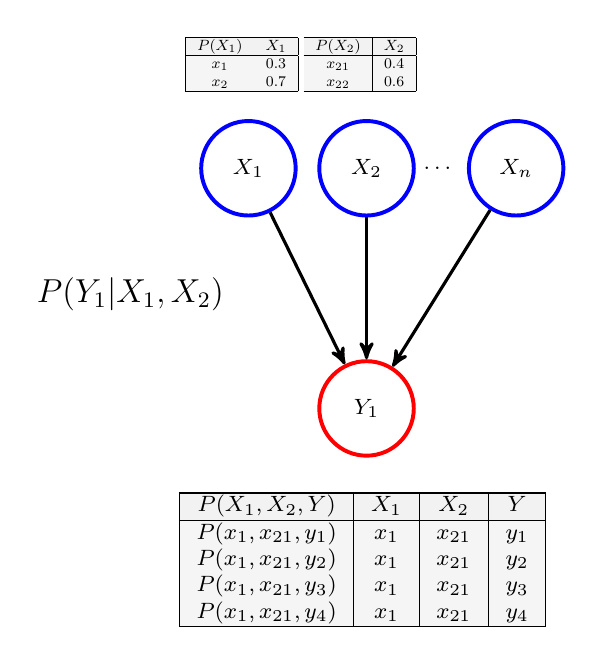
\begin{tikzpicture}[node distance=1.5cm, font=\footnotesize, align=center, >=stealth', line width=0.5mm]
        % Define colors
        \definecolor{lightgreen}{rgb}{0.56, 0.93, 0.56}
        \definecolor{lightred}{rgb}{0.98, 0.5, 0.45}

        % Nodes
        \node[draw, circle, draw=blue, text=black, minimum size=1.2cm] (input1) {$X_1$};
        \node[draw, circle, draw=blue, text=black, right of=input1, minimum size=1.2cm] (input2) {$X_2$};
        \node[right of=input2, node distance=0.9cm] (dots) {$\ldots$};
        \node[draw, circle, draw=blue, text=black, right of=dots, node distance=1cm, minimum size=1.2cm] (inputn) {$X_n$};
        % Probability expression
        \node[left of=input1, node distance=1.5cm, yshift=-1.6cm, font=\large] (prob) {$P(Y_1 | X_1, X_2)$};

        \node[draw, circle, draw=red, text=black, below=1.8cm of input2, minimum size=1.2cm] (output1) {$Y_1$};

        % Edges
        \foreach \i in {1,2,n} {
            \draw[->, line width=0.4mm] (input\i) -- (output1);  % Decreased line width
        }
        \node[above=0.2cm of input1] {
            \resizebox{1.5cm}{!}{%  <-- set the width of the table here
                \begin{tabular}{|c|c|}
                    \hline
                    \rowcolor{gray!10}
                    $P(X_1)$ & $X_1$ \\
                    \hline
                    \rowcolor{gray!8}
                    $x_1$ & 0.3 \\
                    \rowcolor{gray!8}
                    $x_2$ & 0.7 \\
                    \hline
                \end{tabular}
            }
        };

        \node[above=0.2cm of input2] {
            \resizebox{1.5cm}{!}{%  <-- set the width of the table here
                \begin{tabular}{|c|c|}
                    \hline
                    \rowcolor{gray!10}
                    $P(X_2)$ & $X_2$ \\
                    \hline
                    \rowcolor{gray!8}
                    $x_{21}$ & 0.4 \\
                    \rowcolor{gray!8}
                    $x_{22}$ & 0.6 \\
                    \hline
                \end{tabular}
            }
        };
        \node[below=0.3cm of output1] {
            %\resizebox{1.5cm}{!}{
                \begin{tabular}{|c|c|c|c|}
                    \hline
                    \rowcolor{gray!10}
                    $P(X_1, X_2, Y)$ & $X_1$ & $X_2$ & $Y$ \\
                    \hline
                    \rowcolor{gray!8}
                    $P(x_1, x_{21}, y_1)$ & $x_1$ & $x_{21}$ & $y_1$ \\
                    \rowcolor{gray!8}
                    $P(x_1, x_{21}, y_2)$ & $x_1$ & $x_{21}$ & $y_2$ \\
                    \rowcolor{gray!8}
                    $P(x_1, x_{21}, y_3)$ & $x_1$ & $x_{21}$ & $y_3$ \\
                    \rowcolor{gray!8}
                    $P(x_1, x_{21}, y_4)$ & $x_1$ & $x_{21}$ & $y_4$ \\
                    \hline
                    % Rest of the JPD table entries...
                    % ...
                \end{tabular}
            %}
        };        
       
    \end{tikzpicture}
    \caption{\small Graphical representation of BN where nodes $X_i$ represent the input variables and the node $Y_1$ represents the output variable to the deterministic model. The solid lines represent the existing nodes in the model. The double-edged arrow represents additional information.}\label{fig:BN3} 
    %\vspace{-15pt}
\end{figure}

Under the umbrella of ML lies a multitude of computational algorithms, each with their own unique characteristics. Whilst learning, an ML algorithm utilises a statistical model with adjustable parameters that minimises a loss function through adjustment of internal parameters. For instance, in regression tasks, where the algorithm aims to align its output with a target value, common metrics like mean square error are often employed to evaluate its performance. The primary objective of training ML algorithms is to enable predictions for new input data, requiring them to predict outputs for inputs unseen in the training data.

Within ML, BNs represent a unique approach, serving as a type of probabilistic graphical model that encapsulates a set of variables and their conditional dependencies through a directed acyclic graph (DAG)~\cite{Hand2001}. Unlike traditional ML approaches, BNs provide a more explicit representation of probabilistic relationships between variables, facilitating a deeper understanding of the underlying data generating process. This underscores optimising predictive performance to gaining insight into the underlying mechanisms governing the data, making them valuable in real-world, uncertain applications. 

A BN consists of nodes representing variables and edges representing dependencies between variables. The parameters of a BN specify the conditional probabilities associated with each node given its parents in the network. These conditional probabilities determine the relationships and dependencies between variables in the BN.\@ When multiple probability distributions are combined, a Joint Probability Distribution (JPD) is formed. The structure of the Bayesian Network (BN) captures the dependencies between variables, and the conditional probabilities are derived from data or expert knowledge. This allows for the efficient representation of the Joint Probability Distribution (JPD) without explicitly specifying all the individual parameters. Instead, BNs leverage the conditional relations specified by the graph topology, reducing the need to define every parameter explicitly and making them a powerful tool for probabilistic modeling. This provides a compact representation by combining the \textit{local} conditional distributions for each node, with respect to its connected parent nodes~\cite{Koller2009}, see Figure~\ref{fig:BN3}. The joint probability distribution can be factorised into a product of conditional probability distributions, one for each variable given its parents in the graph. This factorisation is known as the chain rule of probability. Also known as the general product rule, this allows the calculation of any member of the joint distribution of a set of random variables using only conditional probabilities.

Given a set of random variables, say $X_1, X_2, \ldots, X_n$, the chain rule of probability states that the joint probability of these variables is the product of the conditional probabilities of each variable given all the variables that precede it. Mathematically, this can be expressed as:

\begin{align}
    P(X_1, X_2, \ldots, X_n) = & P(X_1) \nonumber \\
    & * P(X_2 | X_1) \nonumber \\
    & * P(X_3 | X_1, X_2) \nonumber \\
    & * \ldots \nonumber \\
    & * P(X_n | X_1, X_2, \ldots, X_n-1)
    \label{eq:chain_rule}
\end{align}
    
In Equation~\ref{eq:chain_rule}: $P(X_1, X_2, \ldots, X_n)$ is the joint probability of $X1$ through $Xn$. $P(X_i | X_1, \ldots, X_i-1)$ is the conditional probability of $X_i$ given all the preceding variables.

\begin{figure*}[t]
    \centering
    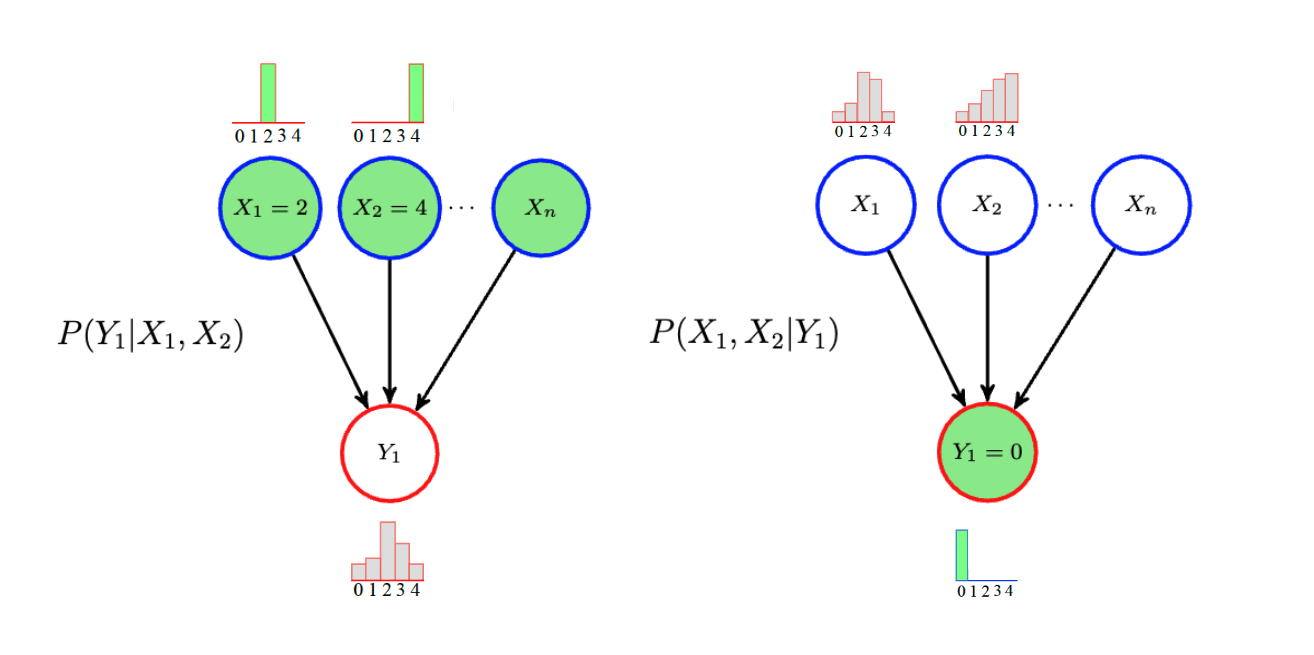
\includegraphics[width=0.75\textwidth]{figures/methodology/inference_F&R_diagram.png}
    \caption{A visual representation of Bayesian inference in the forward (left) and reverse (right) directions.}~\label{fig:inference_F&R_diagram}
\end{figure*}

In depth, the term \textit{prior} refers to the initial probability distribution assigned to a variable. On the other hand, the \textit{posterior} probability refers to the updated probability distribution after \textit{prior} beliefs are updated via \textit{inference}, based on available evidence. The primary benefit of a probabilistic representation lies in its ability to perform \textit{omni-directional inference}, enabling reasoning with uncertain information using probabilistic methods. Thus, adopting a BN as an input-output surrogate model facilitates exploration of causal relationships between fusion parameters and cost in both forward and reverse directions, allowing for an uncertain fusion parameter design space to be mapped from a desired target output range. 

By defining inference as the process of making deductions based on evidence, reasoning and, prior knowledge, it is possible to further characterise Bayesian inference as the act of making alterations to existing probability distributions to discover how, based on their causal relationships, the variable's remaining probability distributions are altered. This acts as a useful tool to measure and understand relationships between inputs and responses in engineering design spaces~\cite{Koller2009}. 

[The interpretation of simulation outputs from analytical models can be challenging for fusion developers without a deep understanding of the associated engineering or physics principles.[discuss w/ Zack]] This can result in reliance on uncertain numerical data, without the ability to leverage the causal structure of the numerical output. In this scenario, a BN can serve as a two-way translation medium between the overall fusion research and the engineering domains. The use of bi-directional inference can assist engineers in providing feedback in the form of design parameters, based on the interconnections between the two domains. In this manner, fusion researchers can impose constraints on the output distributions of the BN, leveraging their expertise and experience, while engineers and physicists handle the input distributions to interpret engineering constraints in terms of design parameters. The `translation' process facilitated by a BN could lead to more comprehensive decisions, as probabilistic inference considers the entire network of relationships between inputs and outputs during computation. This is in contrast to traditional deterministic models, which only consider the direct relationship between inputs and outputs. 

The ability to perform bi-directional inference is a key feature of BNMs, as it allows for the prediction of outputs based on input data, \textit{forward inference}, and inputs based on output data, \textit{reverse inference}. This capability is particularly useful in the context of engineering design, as it enables the exploration of causal relationships between inputs and outputs, and the prediction of inputs based on desired outputs. This can provide valuable insights for decision-making and design optimisation, as it allows for the identification of input values that are most likely to result in a desired output, and the prediction of the likely output given a set of input values. Refer to Figure~\ref{fig:inference_F&R_diagram} for a visual representation of Bayesian inference in the forward (left) and reverse (right) directions. In addition to its flexibility and robustness, the use of Bayesian networks as surrogate models can complement current methods in fusion research by providing a holistic understanding of reactor behaviour and performance. 
    
\subsection{Literature review}~\label{sec:background}

At present, besides the antecedent proof-of-concept study, no known instances exist where BNs have specifically been employed as surrogates in fusion research~\cite{Griffiths2024}. Consequently, this section will delve into the application of ML in fusion research, with a particular focus on the utilisation of other Bayesian modeling techniques in surrogates and uncertainty quantification.

In a review article by Pavonne et al.\ a comprehensive overview of ML and Bayesian inference in fusion R\&D is provided~\cite{Pavone2023}. Bayesian inference facilitates the efficient utilisation of shared information among heterogeneous experimental data sources concerning a common underlying description or model of a phenomenon. The study outlines fundamental Bayesian modeling for fusion experiments in physics models via inference of plasma equilibria~\cite{Svensson2003, Svensson2004}, Gaussian process (GP) tomography~\cite{Svensson2011}, and uncertainty propagation~\cite{Fischer2020, Fischer2010}. The application of ML in fusion research has encompassed various types, demonstrating the potential to address complex challenges in fusion reactor design and operation.[See Zack comment]

Pavone et al.~details significant studies employing trending ML techniques in fusion, particularly within the realm of deep learning (DL) methods in neural networks. Specifically, in the theory of artificial neural network (ANN) algorithms and convolutional neural networks (CNNs), the latter of which was utilised in~\cite{Pavone2019} for the Wendelstein 7-X Stellarator experiment to reconstruct ion and electron temperature profiles from 2D x-ray spectral images. The article underscores the significance of Bayesian inference for neural networks within the fusion community. Reinforcement learning (RL) has been employed in seminal studies for controlling tokamak plasmas~\cite{Degrave2022} and predicting disruptions~\cite{Kates2019}, showcasing applicability to practical tasks in real-time. In~\cite{Degrave2022}, RL enhanced flexibility in plasma control by generating non-linear feedback controllers, thereby simplifying the control system. The RL system learned the control policy through interaction with a simulated environment modeling the dynamic state of the plasma shape and current, magnetic diagnostics sensor data, coil currents, and controller dynamics. In~\cite{Kates2019}, a disruption mitigation system utilizing DL predicts potential disruptions, aiming to reduce thermal loads. The algorithm combines convolutional and recurrent neural networks (CNN and RNN, respectively), trained on data from the JET and DIII-D experiments. The CNN learns the temporal dynamics of the plasma and predicts the likelihood of disruptive states. If the system output exceeds a certain threshold, an alarm triggers the activation of a mitigation action. 


\begin{figure*}[t]
    \centering
    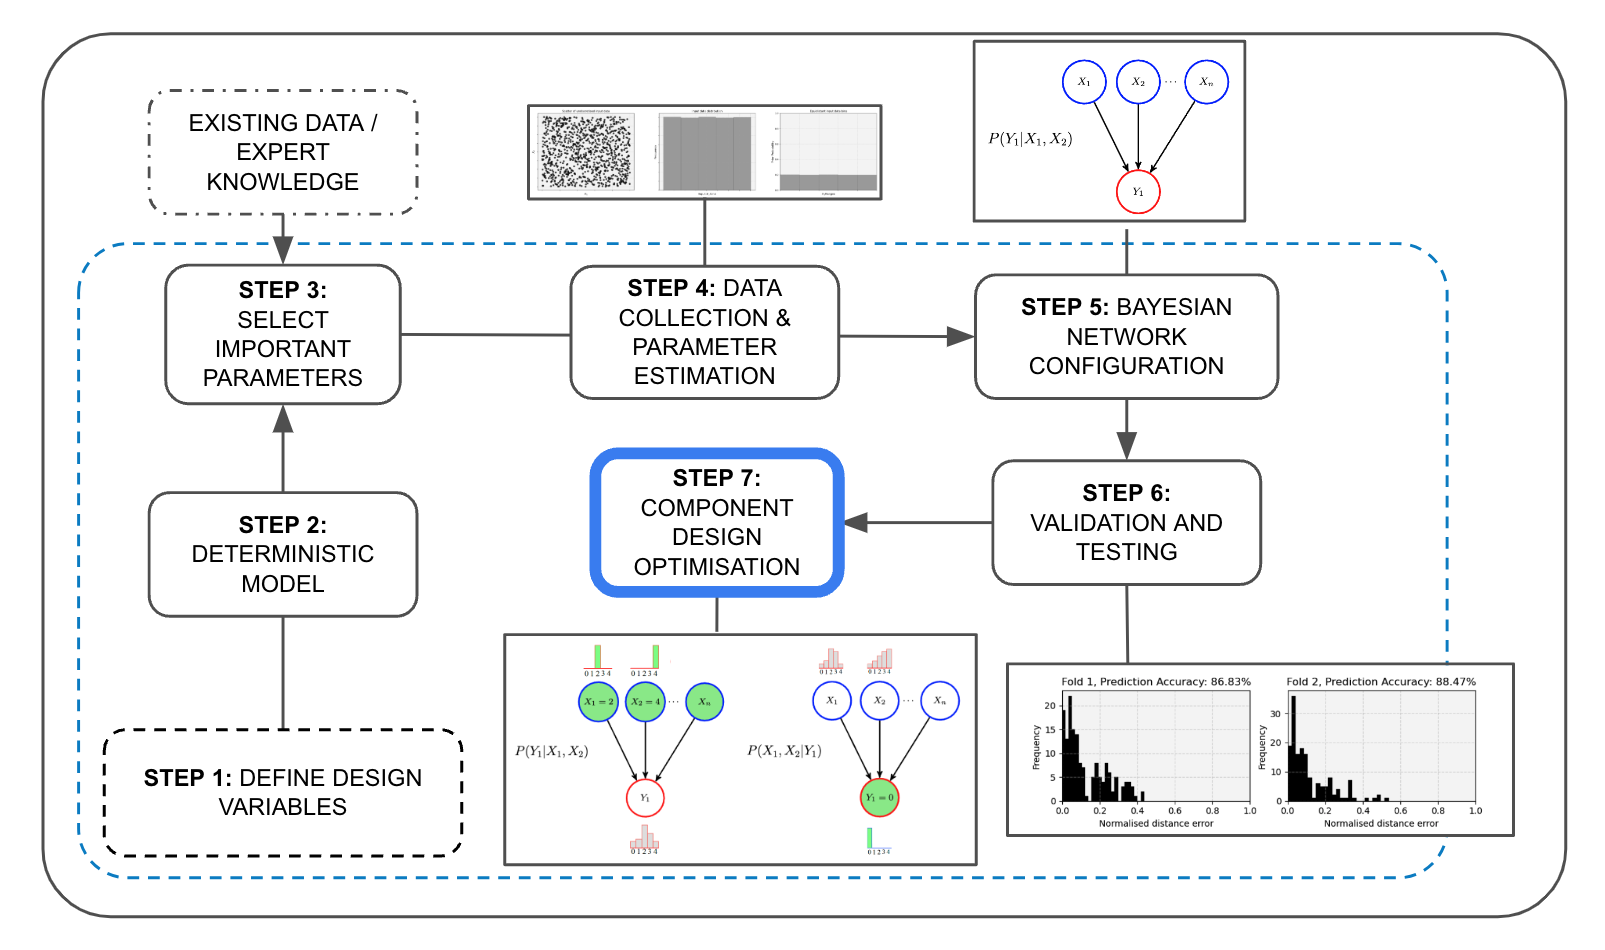
\includegraphics[width=0.9\textwidth]{figures/methodology/workflows/workflow_v5.png}
    \caption{Workflow of the surrogate modelling process, adapted from~\cite{Conti2019}, and refined from the methodology presented in~\cite{Griffiths2024}}~\label{fig:workflow}
\end{figure*}


Surrogate models aim to expedite computationally intensive models based on numerical approximations and theoretical first principles, a particularly crucial endeavor in fusion research, especially concerning turbulent transport computations. An illustrative case provided in~\cite{Van2020} demonstrates the efficacy of surrogate models: leveraging a dataset from~\cite{Citrin2017}, a neural network was trained. Integrated into modeling simulations, this neural network efficiently calculated the evolution of ion and electron temperature profiles as well as electron density profiles. The network delivered crucial values such as the main ion and electron heat flux and electron particle flux at a remarkable speed—864 times faster than a numerical model requiring four times the number of cores. Similar instances of neural networks serving as surrogates can be found in~\cite{Meneghini2017}, focusing on turbulent transport calculations, and~\cite{Miller2021}, exploring physics-informed plasma behaviour in a particle-in-cell gyrokinetic code.

Pavone et al.\ also shed light on the computational complexity inherent in Bayesian inference, particularly in sampling from the posterior distribution. They elucidate that while Markov Chain Monte Carlo (MCMC) methods offer a means to sample from the posterior, their practicality diminishes in many real-world scenarios due to the substantial number of iterations required. The primary bottleneck arises from the need to compute the likelihood function, which entails running a forward models or simulation code—a process often prohibitively slow in complex systems. Pavone and colleagues argue that deep learning (DL) models offer a promising alternative, demonstrating their ability to efficiently reconstruct the posterior and infer plasma parameters from diagnostic data within short time frames, as evidenced in studies such as those by Pavone et al.~\cite{Pavone2018,Pavone2019, Pavone2020, Pavone2021}

In navigating the landscape of fusion research, the interplay between machine learning (ML) techniques and Bayesian inference emerges as a pivotal force, offering novel avenues for addressing complex challenges. While BNs have yet to find widespread application as surrogates in fusion studies, the realm of ML, bolstered by Bayesian modeling techniques, presents a range of possibilities. From the nuanced inference of plasma equilibria to the predictive power of deep learning methods like convolutional neural networks (CNNs), researchers navigate a diverse array of methodologies to elucidate the intricacies of fusion phenomena. As surrogate models expedite computations and DL models offer efficient alternatives to Bayesian networks, the fusion community stands at the precipice of transformative discovery, guided by the symbiotic relationship between traditional methodologies and cutting-edge computational techniques. This study aims to bridge the gap between these two fields, leveraging the power of BNs as surrogate models to combat uncertainty in fusion engineering and drive design optimisation decisions in real-world scenarios.

\section{Methodology}\label{sec:methodology}

In this section, a set of general procedures for creating and applying a BN as a surrogate model is presented, drawing inspiration from~\cite{Conti2019}. Illustrated in Figure~\ref{fig:workflow}, a surrogate modelling framework delineates the creation, cross-validation, and application of the BNM, applicable to various input-output problems. For illustrative purposes, reference is made to the BNM of the PROCESS systems code, presented in the proof-of-concept study~\cite{Griffiths2024}. Each step is explored methodically, focusing on identifying optimal deployment strategies. These include specific hyper-parameters, such as bin resolution, and validation techniques. 

\subsection{\textbf{Step 1}: Define design variables}\label{sec:design}

In this step, a strategic decision is made regarding the focal point of the model, whether it targets a whole reactor system or a critical component such as the breeder blanket or the divertor. Following this decision, the key parameters and characteristics of the chosen component are then identified and defined as input variables, labeled as $X_1$, $X_2$, \ldots, $X_n$. As exemplified in the proof-of-concept study conducted by Griffiths et al.~\cite{Griffiths2024}, this process involved the conceptualization of a future-type spherical tokamak reactor system to conduct a comprehensive investigation into its economic viability. In this study, the inputs and outputs of the model were framed as the design variables, allowing for a holistic evaluation of the power plant's economics.

Ahead of executing the selected deterministic model, it requires configuration. This process includes choosing the inputs and outputs, along with defining the value ranges for each variable. The selection of inputs and outputs is guided by the objectives of the analysis and the data at hand. The value ranges for each variable are set considering the system's physical limitations and the required granularity of the analysis. Once configured, the deterministic model is run to produce the dataset, which is then utilised to set up the BNM.@ When implementing a BN in a surrogate model, the model will perform better at making predictions when the input distribution is uniform. This is for several reasons: model assumptions: normal distributions assume a bell-shaped curve with values concentrated around a mean, while uniform distributions make no assumptions about data shape and better capture the true underlying distribution. Nonlinearity and Outliers: normal distributions are sensitive to outliers, as they can significantly impact the mean and standard deviation, which may not accurately represent the underlying relationship between variables. Uniform distributions, being less influenced by extreme values, can provide a more robust representation of the data. Flexibility and Non-parametric Modelling: Uniform distributions offer flexibility in modelling unknown or non-normally distributed data without relying on specific distribution assumptions, allowing the BN to adapt and capture complex relationships. Simplification of model complexity: normal distributions require additional parameters (mean and standard deviation) that necessitate estimation, increasing model complexity and the number of parameters to learn. In contrast, using uniform distributions simplifies the model by eliminating the need for extra parameter estimation, resulting in easier training and interpretation~\cite{Duda1973,Neapolitan2004, Koller2009}.

\begin{figure*}[t]
    \centering
    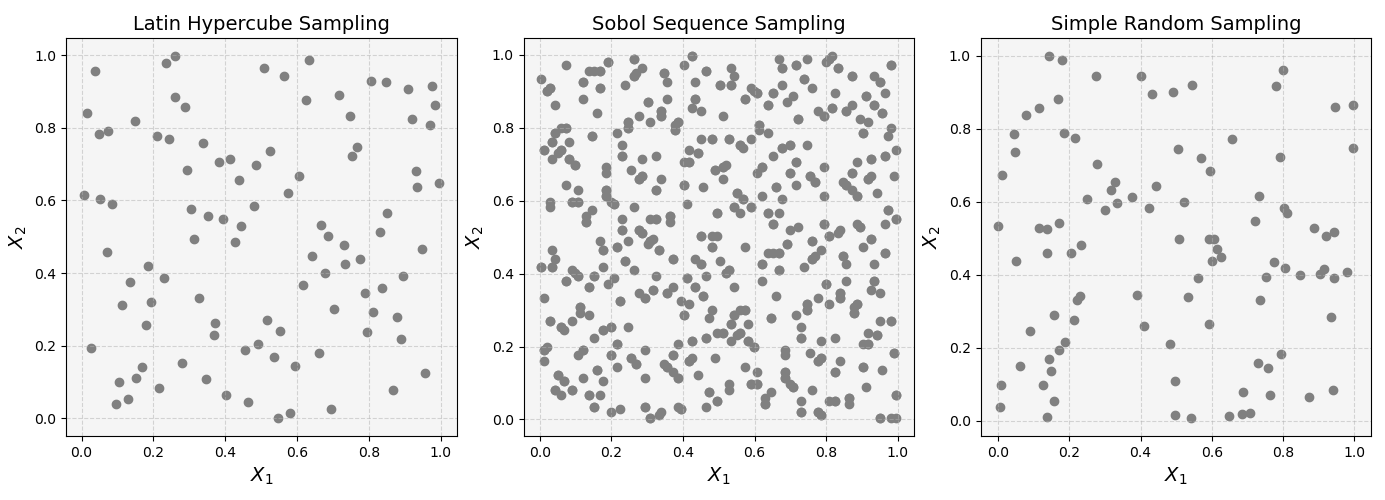
\includegraphics[width=0.8\textwidth]{figures/methodology/sobol_vs_lhs_simple.png}
    \caption{\small A comparison of the Sobol and Latin Hypercube sampling methods.}~\label{fig:sobol_vs_lhs}
\end{figure*}

\subsection{\textbf{Step 2}: Deterministic model}\label{sec:deterministic}


The deterministic model forms the basis of the BNM, integrating various models to emulate a system rather than relying on a singular approach. In the context of fusion research, systems codes incorporate a multitude of models encompassing diverse aspects of reactor behavior, including plasma physics, material properties, neutron transport, and cost estimations. These models collectively form a comprehensive framework for simulating and analysing fusion reactor systems. Its primary function is to generate output variables, denoted as $Y_1$, $Y_2$, \ldots, $Y_m$, which serve as the foundation for data collection and parameter estimation in developing the surrogate model. Drawing from the proof-of-concept study by Griffiths et al.~\cite{Griffiths2024}, an illustrative example of this step involves the utilisation of the UKAEA systems code, PROCESS~\cite{Kovari2014, Kovari2016}. This model examines the interconnection between the engineering and physics subsystems comprising a fusion power plant while accommodating user-defined constraints.

\subsection{\textbf{Step 3}: Parameter Selection}\label{sec:parameters} 
In this stage, the focus is on identifying and selecting input parameters that wield substantial influence over the output variables modeled by the deterministic model. This task demands careful deliberation and expertise to discern the most pertinent parameters governing the system's behaviour and performance.

~\cite{Griffiths2024} illustrates this process. A Spherical Tokamak (ST) design basis was utilised from a previous work by the same authors, presenting a comprehensive techno-economic analysis of ST fusion power plants for hybrid hydrogen-electricity production~\cite{Hidalgo-Salaverri2023}. To lay the groundwork for the techno-economic investigation, which encompassed evaluations under optimistic, moderate, and conservative scenarios, a rigorous sensitivity analysis was conducted. The objective was to streamline the problem's complexity by screening other potentially economically significant parameters.

Inputs were delineated as the reactor's design parameters, including the Greenwald fraction, W impurity fraction, current drive efficiency factor, aspect ratio, toroidal field [T], total plasma beta, NBI plug efficiency, and turbine inlet temperature [ºC]. Outputs, on the other hand, were characterised as the economic parameters of the reactor, such as the capital cost [millions USD\$]. The ranges for each variable were established considering the system's physical constraints, the required level of analysis granularity, and existing values derived from ST design bases documented in the literature.

\subsection{\textbf{Step 4}: Data Collection and Parameter Estimation}\label{sec:data} 

Here, the deterministic model is executed to gather data required to configure the surrogate model. Its imperative to collect comprehensive data representing the entire design space to ensure the surrogate model's accuracy. Specific sampling techniques such as Latin Hypercube or Sobol sampling are employed to ensure the collected data adequately covers the design space. Figure~\ref{fig:sobol_vs_lhs} illustrates the sampling of the input space. The collected data is then utilised to configure the surrogate model. 

For example, the final phase of~\cite{Hidalgo-Salaverri2023} focused on employing a Sobol analysis, which generated the dataset for~\cite{Griffiths2024}. The input space was sampled between the parameter limits using Saltelli's extension of the Sobol sequence~\cite{Sobol2001, Saltelli2002}; a quasi-random low-discrepancy sequence used to generate uniform samples of parameter space~\cite{Herman2023}. This analysis extensively investigated the influence of input parameters on the variance of the output, capital cost, by executing PROCESS $>$10,000 times. The analysis considered first-order ($S_{1}$), second-order ($S_{2}$), and complete interaction effects ($S_{\text{tot}}$), thus identifying key economic parameters and their interrelationships, conceptualising the design space of the nodes for the BN.\@

\subsection{\textbf{Step 5}: Bayesian Network Configuration}\label{sec:BNconfiguration}

\begin{figure*}[t]
    \centering
    \begin{minipage}{\textwidth}
        \begin{subfigure}{\textwidth}
            \centering
            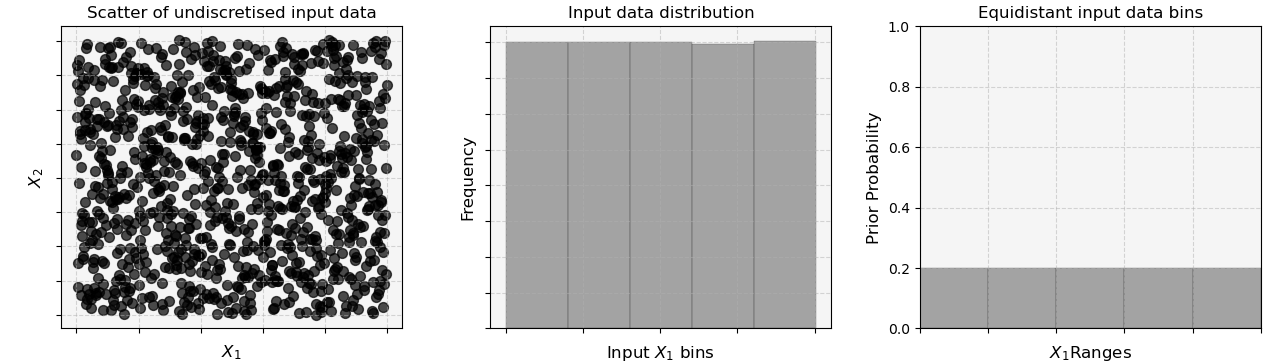
\includegraphics[width=0.7\textwidth]{figures/TE_results/march_data/equidistant_binning.png}
            \caption{\small inputs}\label{fig:input_dist_eg}
        \end{subfigure}
    \end{minipage}
    \begin{minipage}{\textwidth}
        \begin{subfigure}{\textwidth}
            \centering
            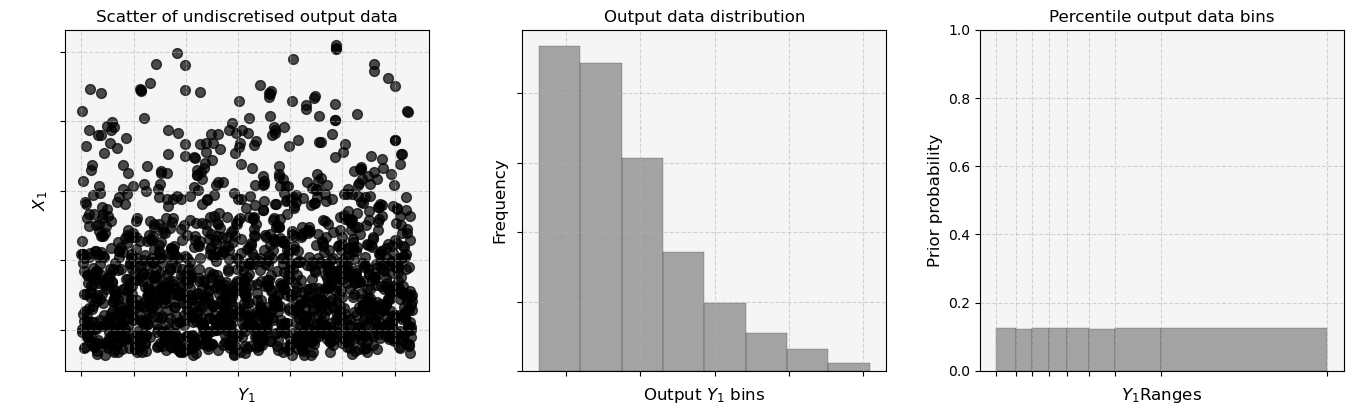
\includegraphics[width=0.7\textwidth]{figures/TE_results/march_data/percentile_binning.png}
            \caption{\small outputs}\label{fig:output_dist_eg}
        \end{subfigure}
    \end{minipage}
    \caption{\small An example of the distribution of a variable demonstrating transformation to equidistant (a), and percentile (b) binning for inputs and outputs, respectively.}\label{fig:dists_eg}
\end{figure*}

The BN is configured at this stage to emulate the deterministic model, using the inputs selected in Step~\ref{sec:parameters} and the data collected in Step~\ref{sec:data}. The data is discretised either by equidistant binning or by percentiles, for inputs and outputs respectively.

BNs are designed to handle discrete distributions, which means that datasets need to be discretised into bins before they can be used. This discretisation process is necessary to convert continuous data into discrete categories or intervals that the BN can handle effectively. By discretising the dataset into appropriate bins, the BN can leverage the discrete nature of the variables and make probabilistic inferences. Discretisation is a method used in machine learning to transform continuous variables into discrete categories or bins.

For example, in~\cite{Griffiths2024}, two distinct methods of discretisation were employed: \textit{equal distance} and \textit{percentile binning}. For the inputs, the \textit{equal distance} approach was applied, while the \textit{percentile binning} method is implemented for the target (output). This differentiation allows for an effective and tailored discretisation process that accommodates the specific characteristics and requirements of the inputs and outputs.

Equal distance binning divides the range of a variable into a fixed number of equal-sized intervals or bins\@. This method assigns values to bins based on their proximity to the bin boundaries. Equal distance binning is commonly used for discretising input features in machine learning because it preserves the linear relationship between the variable values and allows for easy interpretation of the results. It can be particularly useful when the variable exhibits a linear trend or when the absolute values of the variable are important for the prediction task, making it the most appropriate method during the initial construction of the BN.\@ Referring to Figure~\ref{fig:input_dist_eg}, the input distribution of a variable demonstrates the need for equidistant binning.

On the other hand, percentile binning divides the data based on the distribution of the variable values. Each bin contains an equal number or percentage of data points, ensuring that the bins capture an approximately equal amount of information. Percentile binning is often preferred for discretising target or output variables in ML.\@ This is because output data distributions are typically less uniform. It can thus help handle class imbalance issues, i.e., bias, and create more balanced categories for classification tasks. By grouping data points based on their relative positions in the distribution, percentile binning can ensure that each bin represents a similar portion of the target variable, reducing the impact of outliers and enhancing model performance. Referring to Figure~\ref{fig:output_dist_eg}, the input distribution of a variable demonstrates the need for equidistant binning.  Overall, the selection of the appropriate discretisation method should be based on an understanding of the data distribution, the specific machine learning task, and the goals of the analysis. 

Once discretised into probability distributions, both input and output data from training dataset are used determine the structure of the BN.~This is done by establishing relationships between variables according to the information provided by the training data. Here the BN learns the parameters and develops the causal relationships between them, i.e., populates the conditional probability tables with the prior distributions of the variables. In this context, the pre-configured and validated BN can then be employed to perform bi-directional inference in Step~\ref{sec:meth_decision}.

\subsection{\textbf{Step 6}: Model Validation and Testing}\label{sec:meth_validation} 

Here details the implementation of Step~\ref{sec:meth_validation} using the dataset from the proof-of-concept study~\cite{Griffiths2024}. Specifically, this section provides an overview of the outcomes obtained through $k$-fold cross-validation, and presents the findings from hyper-parameter tuning. The validation process was conducted to assess the BN's predictive accuracy and reliability, and to identify the optimal hyper-parameters for configuring the model. The results of the validation process provide valuable insights into the performance of the BNM and inform the selection of hyper-parameters for future model development.

Validation is the term used to measure model accuracy. As part of the validation procedure and in order to avoid bias, a partitioning technique was used to partition the dataset into training and testing in $k$ distinct manners, known as $k$-fold cross-validation. This means the BN was built, and then validated $k$ times, with $k$ unique combinations of training and $k$ testing sets. The ratio of the split between training and testing sets in each fold is determined by the number of folds used to split the dataset by $1/k$, e.g., 3 folds will have a test split size of $1/3 = 33\%$. 

In order to quantify how well the model makes predictions compared to the deterministic response, the predicted values were compared with the actual values in the testing data. In traditional machine learning evaluation methods like Root Mean Square Error (RMSE), the predictions and actual values are typically scalar values, such as numerical measurements or continuous variables. However, in the context of BNs, the outputs are probabilistic, distributions, or categorical variables rather than single numerical values. As a result, standard evaluation metrics like RMSE are not directly applicable, and alternative or custom approaches must be used to assess the performance of BNMs. This is done through calculation of a Normalised Distance Error (NDE), which is the either: the difference between the mean of the predicted bin and the simulated value in the testing data (referred to as $d_{1}$ errors), the difference between the mean of the predicted bin and the mean of the bin in which the actual simulated value lies (referred to as $d_{2}$ errors).

The NDE is a measure used to assess the relative magnitude of the distance error in relation to the range of values in a given bin. It helps to put the distance error into perspective and make it comparable across different bin ranges. By dividing the distance error by the difference between the maximum and minimum bin range values, a normalised distance error is obtained that takes into account the scale and range of the data. This normalisation allows for a fair comparison of the distance error across different bin ranges, providing a standardised measure of the error~\cite{Conti2019}.

\begin{figure*}
    \centering
    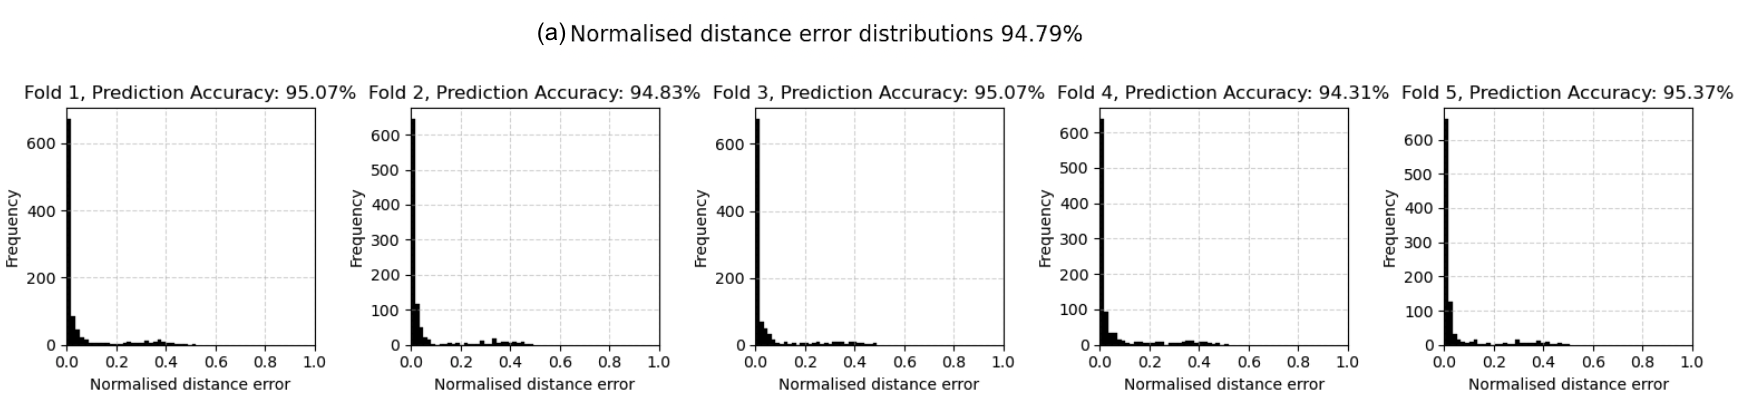
\includegraphics[width=\textwidth]{figures/validation_plots/PROCESS/st20_d1_7bins_folds.png}
    \caption{\small Normalised probability histograms for the proof-of-concept surrogate in~\cite{Griffiths2024}, with prediction accuracy values for the first 5 folds is shown for $d_{1}$ bin resolution = 7, dataset size = 10240.}~\label{fig:k-foldhistograms}
\end{figure*}


Using the data, calibration of hyper-parameters (such as bin resolution and dataset sizes) were examined by exploring two factors: (i) utilising three distinct dataset sizes and, (ii) experimenting with different bin resolutions during discretisation. The objective was to determine how modifying these parameters impacted the BN's ability to make predictions that could be usefully interpretted by the user. Consequently, for (i) this meant dataset sizes of 1400, 5120, and 10240 and, for (ii), incrementally increasing the number of bins used in discretisation between inputs and outputs for all combinations between 3 and 12, respectively. For (i), it was found that configuring the BN using the largest dataset resulted in the highest prediction accuracy. For (ii) the findings are presented in Figure~\ref{fig:3D_SA_trimmed_39_D1}, illustrating the sensitivity of the prediction accuracy to the bin resolution. It follows that the model exhibited optimal performance when and input data was discretised into 7 bins and output data into 5 bins, respectively. In general, the average prediction accuracy for $d_{2}$ errors tends to be higher than that for $d_{1}$ errors, except in the case of using high bin resolutions.

To enable $k$-fold cross-validation, the dataset was split into 10 folds. 10 fold cross-validation aligns with the recommendation by Marcot et al.~\cite{Marcot2021}, who support the prevalent use of $k$=10 for BNs in literature. Plotting the NDE in a histogram provides a good illustration of model performance, see Figure~\ref{fig:k-foldhistograms}. The resulting validation plot distributions in Figure~\ref{fig:k-foldhistograms} offers a clear representation of the model's predictive capabilities. Overall, when observing the distribution of the d1 plots for all 10 folds, it can be noted that the BNM built on 10,000 data points, seems to predict the correct response with an average $\sim$95\% accuracy.

This high level of accuracy underscores the model's robustness and reliability in making predictions. It also highlights the value of using a substantial dataset for building the model, as in~\cite{Griffiths2024}. These findings contribute to the growing body of evidence supporting the use of BNs in making accurate predictions, and they underscore the importance of careful model construction and validation.

The results from the hyper-parameter calibration provide valuable insights into the performance of the BNM.~Two key factors were examined: dataset size and bin resolution during discretisation, refer to Table~\ref{tab:prediction_accuracy}. The investigation found that the size of the dataset used to configure the BN significantly impacts its predictive accuracy. Specifically, the largest dataset (10,240) yielded the highest prediction accuracy. This suggests that the BNM benefits from a larger volume of data, likely because it provides a more comprehensive representation of the underlying distributions and dependencies. Whilst this is not a groundbreaking realisation, it is a useful reminder that the quality of the data used to configure the BN is crucial to its performance. The findings also underscore the significance of acquiring a substantial volume of data to uphold the model's accuracy and reliability, while simultaneously averting overfitting to the training data. Acknowledging that generating sufficient data for a reliable BNM may pose challenges in real-world applications, the utilisation of coarse sensitivity analysis, such as the one carried out prior to the proof-of-concept~\cite{Griffiths2024,Hidalgo-Salaverri2023} or experimental design strategies emerges as an effective approach to mitigate the data volume needed for training. These strategies allow for more efficient use of available data, ensuring robustness and applicability of the BNM in practical engineering scenarios within fusion development. Going forward, this study will inform the collection of data for future BNMs, ensuring that the dataset is sufficiently large to support accurate and reliable predictions, especially when the model is used to make critical decisions in engineering design with fusion developers.

The bin resolution during discretisation also played a crucial role in the BNM's performance. The optimal performance was observed when the input data was discretised into 7 bins and the output data into 5 bins, see Figure~\ref{fig:3D_SA_trimmed_39_D1}. This indicates the necessity of striking a balance in bin resolution. Too few bins may oversimplified the data, resulting in the loss of important information, while an excessive number of bins lead to overfitting, where the BNM became overly tailored to the training data and performed poorly on new data. The choice of hyper-parameters is heavily influenced by the nature of the problem at hand. While formulating universal guidelines is challenging, several rules of thumb emerge from observations across various problems. For instance, if the input-output mapping is highly nonlinear, employing more bins on the output is advisable to capture the high variability. Conversely, if the input space is sparsely sampled, coarser bins are likely necessary. These insights inform the selection of hyper-parameters, ensuring the BNM's effectiveness and robustness across diverse engineering applications in fusion development.

\begin{figure}[h]
    \centering
    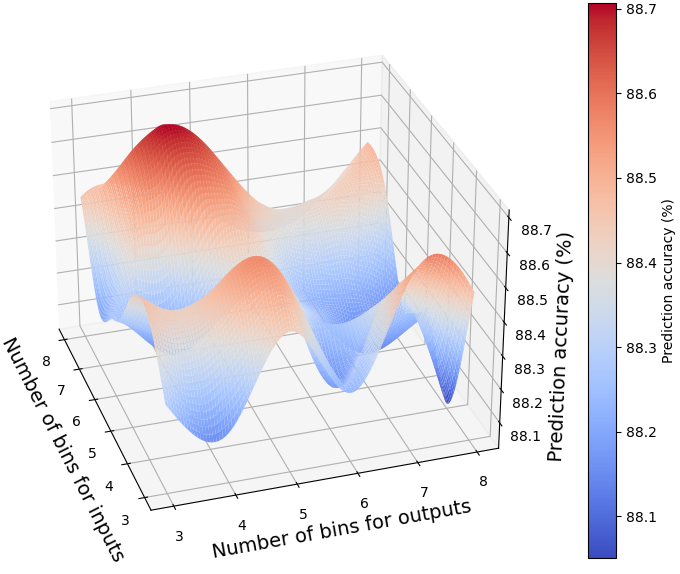
\includegraphics[width=0.9\columnwidth]{figures/validation_plots/PROCESS/SA_3D_trimmed_39.png}
    \caption{\small A 3D surface plot displaying the average accuracy of predictions for $d_{1}$ errors while investigating variations in bin resolution.}~\label{fig:3D_SA_trimmed_39_D1}
\end{figure}

The average prediction accuracy for $d_{2}$ errors was generally higher than that for $d_{1}$ errors, except when using high bin resolutions. This is largely down to how the model handles the different types of errors. The $d_{1}$ error measures the difference between the mean of the predicted bin and the simulated value in the testing data, while the $d_{2}$ error measures the difference between the mean of the predicted bin and the mean of the bin in which the actual simulated value lies. Thus, the likelihood that the correct bin is predicted is higher for $d_{2}$ errors, as it is based on the mean of the bin rather than the actual value. This is an important consideration when interpreting the results and understanding the model's performance. The results suggest that the model may be more sensitive to the bin resolution for $d_{1}$ errors, and care should be taken when choosing the bin resolution in this case.

These findings contribute to a deeper understanding of how hyper-parameter choices affect the performance of BNMs, and can guide the selection of these parameters in future work by providing a clear indication of the optimal dataset size and bin resolution to benchmark the model. This will help to ensure that the BNM is configured to provide accurate and reliable predictions, and that the results can be interpreted with confidence.

\subsection{\textbf{Step 7}: Design Constraint Decision Support}\label{sec:meth_decision}

In this step application of the BN to provide decision support for engineering design is implemented through Bayesian bi-directional inference. Forward inference involves updating prior assumptions of inputs, utilising available evidence to give the output response. Conversely, reverse inference involves estimating the inputs given the output. The ability to perform reverse inference stems from the fact that once a BNM has learned the parameters, it no longer differentiates between inputs and outputs. This characteristic allows the network to infer in both directions, making it possible to predict inputs based on output data., such as determining input ranges for optimal performance based on a desired output using reverse inference. 

\section{Application of the Methodological Framework: Tokamak Energy ST Scenario}\label{sec:res_decision} 

In this section, the BNM is applied to a real-world design phase ST scenario using the methodological framework outlined in~\ref{sec:methodology} to demonstrate its utility in providing decision support for engineering design, where engineers and researchers need to identify the input parameters that will yield the desired output performance. Section~\ref{sec:res_reverse} delves into the outcomes of reverse inference with the BNM, emphasising the prediction of ranges for economic fusion parameters from uncertain data. Results can provide decision support for components, such as determining input ranges for optimal performance based on a desired output using reverse inference. This demonstrates an update from the proof-of-concept with greater depth and analysis given in Step 7 (\ref{sec:meth_decision}). It should be mentioned that the reactor emulated in the PyTOK model is a ST fusion power plant, and firmly in the design phase i.e., pre-first-of-a-kind (FOAK). As a result, some design points did not produce net electricity. This departs from the reactor emulated in the proof-of-concept study~\cite{Griffiths2024}, which was a future-type reactor that met specific design constraints to those necessary of a more mature design that fits in to a future energy system.

For \textbf{Step 1}: Define Design Variables (\ref{sec:design}), the aim was to model a whole reactor system, determining how important output parameters vary with certain inputs by studying their sensitivity to one another. For \textbf{Step 2}: (~\ref{sec:deterministic}), the deterministic  model used was `PyTOK', a systems code that finds optimum working point using a series of 0D and 1D approximations that model all subsystems. For \textbf{Step 3}: (\ref{sec:parameters}), the important parameters for the BNM were carefully selected based on insights from the PyTOK model, a comprehensive tool for fusion reactor analysis.

% Please add the following required packages to your document preamble:
% \usepackage{booktabs}
\begin{table}[]
    \begin{tabular}{@{}llll@{}}
    \toprule
    \textbf{Parameter}       & \textbf{Symbol} & \textbf{Min-Max Range} & \textbf{Units} \\ \midrule
    \multicolumn{4}{c}{\textbf{Inputs}}                                                    \\ \midrule
    Major Radius             & $R$               & 3.0209-3.9988          & (m)            \\
    Aspect Ratio             & $A$               & 1.7990-2.4938          &                \\
    Effective Ion Charge     & $Z_{\text{eff}}$  & 1.1981-2.4976          &                \\
    Toroidal Field on Plasma & $B_{\text{T}}$    & 4.0545-5.9988          & (T)            \\ \midrule
    \multicolumn{4}{c}{\textbf{Outputs}}                                                   \\ \midrule
    Net Electrical Output    & $E$               & -536-140               & (MWe)          \\
    High Grade Waste Heat    & $H$               & 89-769                 & (MWt)           \\
    Capital Cost             & $C$               & 3427.12-8448.38        & USD \$ Million \\ \bottomrule
    \end{tabular}
    \caption{Input and output ST scenario design variables, along with their corresponding minimum and maximum ranges and units}~\label{tab:params}
    \end{table}

The chosen input parameters include: 

\textbf{Major Radius ($R$)} denotes the distance from the center of the toroidal fusion device to the center of the plasma. Its significance in economic fusion, particularly concerning the commercialisation of STs, stems from several key factors.

A larger major radius typically corresponds to a larger plasma volume, which can accommodate greater quantities of fusion fuel and facilitate more efficient energy production. With STs, optimising the major radius becomes essential for achieving economies of scale and maximizing energy output while minimizing capital and operational costs.

The major radius influences key plasma stability characteristics crucial for sustained fusion reactions. By providing sufficient space for plasma confinement, a larger major radius helps mitigate instabilities and turbulence within the plasma, thereby enhancing overall fusion performance and reactor reliability.

Moreover, from an economic standpoint, the major radius impacts reactor engineering and infrastructure costs. While larger major radii may entail higher initial investment costs for reactor construction, they often result in improved fusion performance, higher energy output, and potentially lower operational costs per unit of electricity generated. Therefore, optimizing the major radius in ST designs involves striking a balance between upfront capital expenditures and long-term economic viability, with the aim of achieving competitive electricity prices in the energy market.

\begin{figure*}[t]
    \centering
    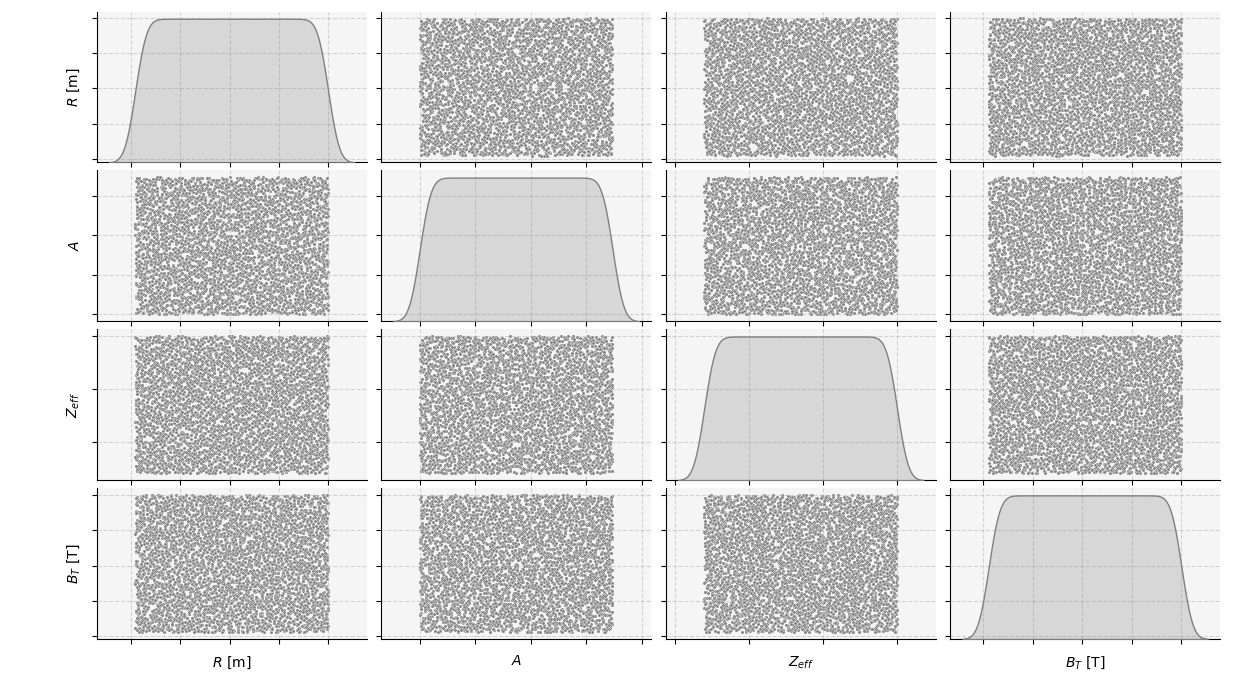
\includegraphics[width=0.8\textwidth]{figures/TE_results/4x4scatter_inputs_marchdata.png}
    \caption{\small A 4$\times$4 scatter-grid to illustrate the sampling of the deterministic input space. The scatter-grid is a visual representation where each point represents a unique combination of input values}\label{fig:scatter_sampling}
\end{figure*}

\textbf{Aspect Ratio ($A$)} is a fundamental parameter in fusion reactor design, representing the ratio of the $R$ to the minor radius ($a$) of the plasma confinement region. In the context of fusion physics, particularly within the domain of STs, higher aspect ratios are characteristic features.

The aspect ratio holds significant importance in shaping the equilibrium and dynamics of the plasma within the fusion device. Specifically, it influences plasma stability and confinement properties, with higher aspect ratios typically associated with enhanced plasma stability and improved confinement characteristics~\cite{Costley2019}.

\textbf{Effective Ion Charge ($Z_{\text{eff}}$)}: This parameter serves as a metric for the average charge state of ions, reflecting the balance between the positively charged ions and the negatively charged electrons within the plasma. This charge state is determined by summing the squares of the charges of individual ion species present in the plasma, each weighted by their respective densities.

\begin{equation}
    Z_{\text{eff}}=\frac {\sum _{i}n_{i}Z_{i}^{2}}{\sum _{i}n_{i}Z_{i}}
\end{equation}

where $n_{i}$ is ion density for species $i$ and $Z_{i}$ is the charge state of species $i$. $\sum _{i}n_{i}Z_{i}=n_{e}$ by quasi-neutrality, so

\begin{equation}
    Z_{\text{eff}}=\frac {\sum _{i}n_{i}Z_{i}^{2}}{n_{e}}
\end{equation}

In an ideal scenario where a plasma is made up solely of hydrogen isotopes, the effective charge state, $Z_{\text{eff}}$, would be 1. However, in real-world conditions, $Z_{\text{eff}}$ tends to be higher due to the presence of impurities originating from components facing the plasma.

A higher effective ion charge suggests a greater predominance of higher charge states among the ions in the plasma. This can occur due to various factors, including the presence of impurities or the specific conditions within the fusion device. Impurities, such as trace elements or contaminants introduced into the plasma, can significantly influence the effective ion charge by contributing additional charge states to the overall distribution.

In carbon-walled tokamaks, a typical starting point for $Z_{\text{eff}}$ is 2~\cite{Carlstrom1999, Eich2011}. Some comprehensive databases limit their scope to scenarios with relatively low $Z_{\text{eff}}$ values~\cite{Schissel1988}, rendering their scaling laws applicable for $Z_{\text{eff}}<3$ and potentially unreliable for greater $Z_{\text{eff}}$ values. The ITER physics basis from 1999 projects $Z_{\text{eff}}$ to be between 1.8 and 1.9~\cite{ITER19991, ITER19994}, as exceeding this range could lead to excessive fuel dilution.

\textbf{Toroidal Field on Plasma ($B_{\text{T}}$)} holds particular significance in the context of STs due to its pivotal role in plasma confinement and stability. In STs, the toroidal field serves as a critical mechanism for confining the plasma along the toroidal direction, which is essential for maintaining its shape and preventing it from contacting the chamber walls. This confinement is crucial for sustaining the high temperatures and pressures necessary for nuclear fusion reactions to occur.

One of the primary functions of the toroidal field in STs is to counteract the outward forces exerted by the plasma's thermal pressure, gravitational forces, and centrifugal effects. By generating a strong magnetic field that wraps around the torus in the direction of the major radius ($R$), the toroidal field effectively confines the plasma within the central region of the device. This confinement prevents the plasma from expanding radially outward and ensures that it remains tightly contained within the magnetic confinement structure.

Furthermore, the strength of the toroidal field directly influences the stability and performance of the plasma in STs. A sufficiently strong toroidal field helps to suppress instabilities and turbulence within the plasma, which can disrupt fusion reactions and degrade overall performance.

The chosen output parameters were:

\textbf{High Grade Waste Heat ($H$) (MWt)}: $H$ refers to the thermal energy harnessed in a thermodynamic cooling cycle by the breeder blanket for efficient conversion into usable heat or electricity. The heat can also be utilised for various industrial processes, district heating, or power generation, maximising the reactor's energy output and overall efficiency~\cite{Griffiths2022}. Efficient utilisation of waste heat maximizes the overall efficiency of the fusion reactor if non-electric applications can be implemented alongside electricity generation~\cite{Hidalgo-Salaverri2023}.

\textbf{Net Electrical Output ($E$) (MWe)}: This parameter quantifies the amount of electrical power generated by the fusion reactor. Achieving a high $E$ signifies the effectiveness of the fusion reaction in producing usable electrical energy. Thus, an elevated $E$ can contribute significantly to the grid, meeting energy demands to provide baseload power and ultimately reducing reliance on fossil fuels or other non-renewable sources. 

\textbf{Capital Cost ($C$) (million USD)}: This represents the overnight cost of building the fusion reactor. It is a crucial factor in assessing the economic feasibility and viability of implementing fusion energy technology. 

\begin{figure}[t]
    \centering
    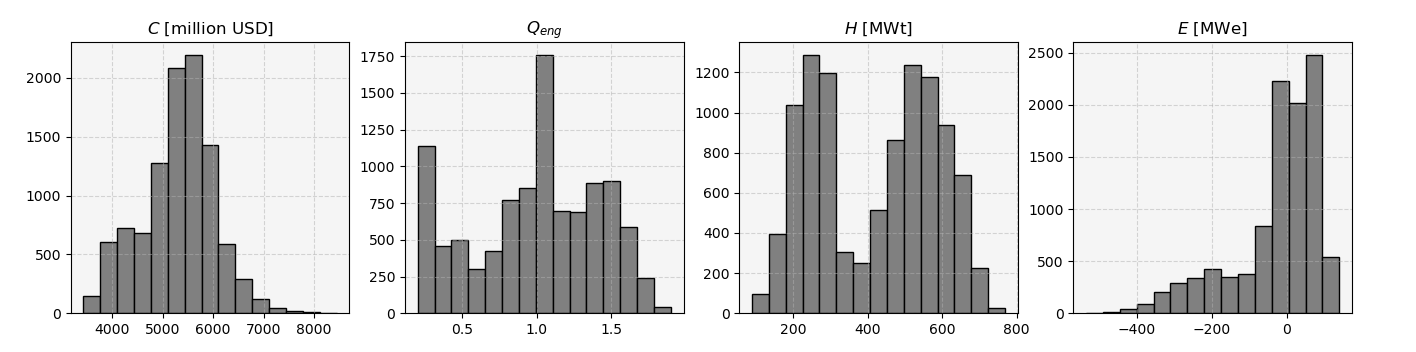
\includegraphics[width=\columnwidth]{figures/methodology/output_distributions.png}
    \caption{\small Histograms of the output variables from the deterministic model.}~\label{fig:outputs_marchdata}
\end{figure}

For \textbf{Step 4}: (\ref{sec:data}), the input space between the parameter limits was sampled using the identical Sobol methods to that in\cite{Griffiths2024}. Data was sampled from the inputs and collected from the PyTOK model to produce a dataset size of 10,420. See Figure~\ref{fig:scatter_sampling} for detailed diagram of the sampling space between the input parameters listed in Table~\ref{tab:params}. See Figure~\ref{fig:outputs_marchdata} for histograms showing the distribution of the output parameters. $H$ shows a multi-modal distribution, typically an indication of high non-linearity in the modelling between inputs and outputs. 
For \textbf{Step 5}:,~\ref{sec:BNconfiguration}, the BN was configured to emulate PyTOK using the inputs outlined in above for~\ref{sec:parameters}, see Figure~\ref{fig:BN2}. The data was discretised using the optimal bin resolution of 7 for the inputs and 5 for the outputs, as determined in the hyper-parameter calibration. The BN was then validated using 10(k)-fold cross-validation to assess its predictive accuracy and reliability. The validation process provided valuable insights into the performance of the BNM and informed the selection of hyper-parameters for future model development. See the Appendix~\ref{appendix:prediction_accuracy} Figure~\ref{fig:k-foldhistogramsTE}.

\begin{figure}[t]
    \centering
    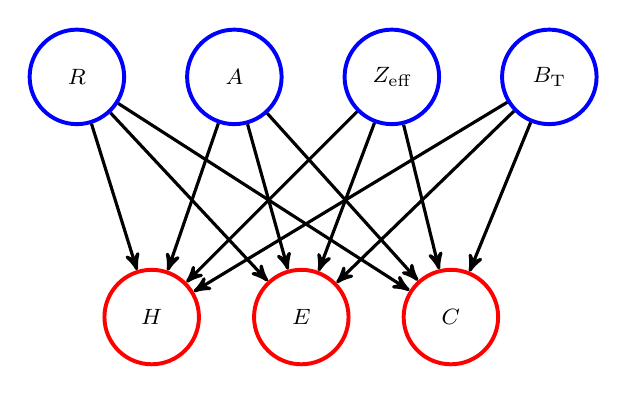
\begin{tikzpicture}[node distance=1.5cm, font=\footnotesize, align=center, >=stealth', line width=0.5mm]
        % Define colors
        \definecolor{lightgreen}{rgb}{0.56, 0.93, 0.56}
        \definecolor{lightred}{rgb}{0.98, 0.5, 0.45}

        % Nodes
        \node[draw, circle, draw=blue, text=black, minimum size=1.2cm] (input1) {$R$};
        \node[draw, circle, draw=blue, text=black, right of=input1, xshift=0.5cm, minimum size=1.2cm] (input2) {$A$};
        \node[draw, circle, draw=blue, text=black, right of=input2, xshift=0.5cm, minimum size=1.2cm] (input3) {$Z_{\text{eff}}$};
        \node[draw, circle, draw=blue, text=black, right of=input3, xshift=0.5cm, minimum size=1.2cm] (input4) {$B_{\text{T}}$};

        \node[draw, circle, draw=red, text=black, below=1.8cm of input2, xshift=-1.05cm, minimum size=1.2cm] (output1) {$H$};
        \node[draw, circle, draw=red, text=black, below=1.8cm of input2, xshift=0.85cm, minimum size=1.2cm] (output2) {$E$};
        \node[draw, circle, draw=red, text=black, below=1.8cm of input2, xshift=2.75cm, minimum size=1.2cm] (output3) {$C$};
        % \node[draw, circle, draw=red, text=black, below=1.8cm of input2, xshift=3.15cm, minimum size=1.2cm] (output4) {$Q_{\text{eng}}$};

        % Edges
        \foreach \i in {1,...,4} {
            \foreach \j in {1,...,3} {
                \draw[->, line width=0.4mm] (input\i) -- (output\j);  % Decreased line width
            }
        }
    \end{tikzpicture}
    \caption{\small Graphical representation of the configured Bayesian Network where nodes represent the input variables (Major Radius ($R$), Aspect Ratio ($A$), Effective Ion Charge ($Z_{\text{eff}}$), Toroidal Field on Plasma ($B_{\text{T}}$)) and the output variables (High Grade Wasteheat ($H$), Net Electrical Output ($E$), and Capital Cost ($C$)) to the deterministic model.}\label{fig:BN2} 
    \vspace{-15pt}
\end{figure}

%%\subsection{Forward Inference}\label{sec:res_forward}
\subsection{\textbf{Reverse Inference}}\label{sec:res_reverse}

\begin{figure*}[t]
    \centering
    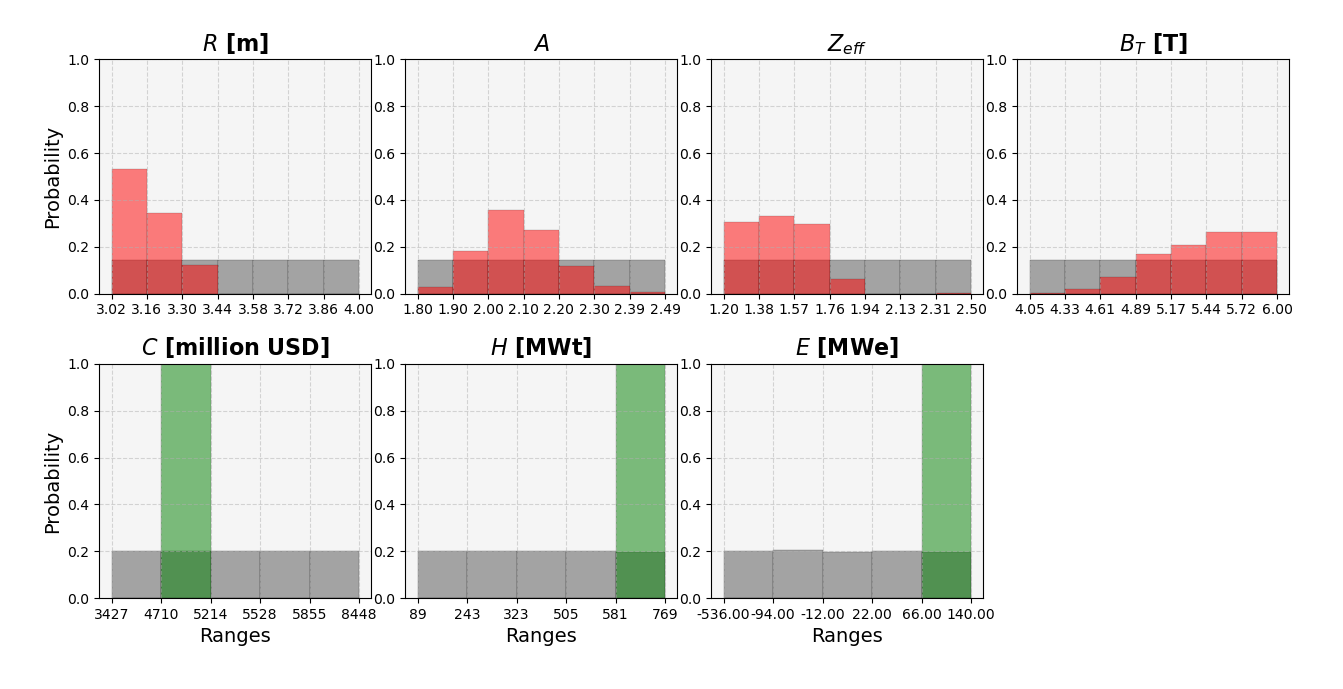
\includegraphics[width=0.80\textwidth]{figures/TE_results/march_data/config(57)_3outputs_v2_6.png}
    \caption{\small Posterior distributions, highlighted in red, of input parameters with fixed $C$ (\$5.2--5.8 billion), $E$ (66--140[MWe]), and $H$ (581--769[MWt]).}~\label{config(57)_outputs(4)3_eg}
\end{figure*}

Corresponding to \textbf{Step 7} in~\ref{sec:methodology}, this section presents the outcomes of reverse inference, employed to predict the input parameters that are most likely to yield a specified output, such as minimising $C$. In doing so the model is able to constrain input parameters and optimise power plant design. The results are presented in distinct sections, each focusing the impact of varying different output parameters ($H$, $E$, and $C$) on input parameters ($R$, $A$, $Z_{\text{eff}}$, and $B_{\text{T}}$).

When a posterior probability (depicted in red) surpasses the corresponding prior probability (shown in grey), it signifies a higher likelihood of the value and is therefore noteworthy (unless the posteriors are uniformly distributed across the entire range). In cases where multiple posteriors exceed the prior, these are identified as the most probable range, provided the bins are contiguous. A posterior probability exceeding 0.5 is considered the most probable value and is explicitly stated as such. Where the highest posteriors are seen at opposite ends of the range, this is noted as a multimodal distribution. A multimodal distribution indicates that the input parameter is sensitive to the output parameter and may exhibit different behaviours depending on the output value. In this case, hybrid evidence analysis is required to determine the most probable range. This requires placing evidence on the multimodal parameter and removing evidence on the output parameter to ascertain the most probable range.   

An example illustating reverse inference is provided in Figure~\ref{config(57)_outputs(4)3_eg}. Here, the posterior distributions (red) of the input parameters are shown with fixed $C$ (\$5.2--5.8 billion), $E$ (66--140[MWe]), and $H$ (581--769[MWt]) (green). For further depth in the analysis, it was necessary to fix certain output parameters to observe the sensitivity of the input parameters posterior probability distributions through plotting multiple posteriors for each input parameter. To visualise this, see~\ref{fig:posterior_planes3}.


% \begin{figure*}[t]
%     \centering
%     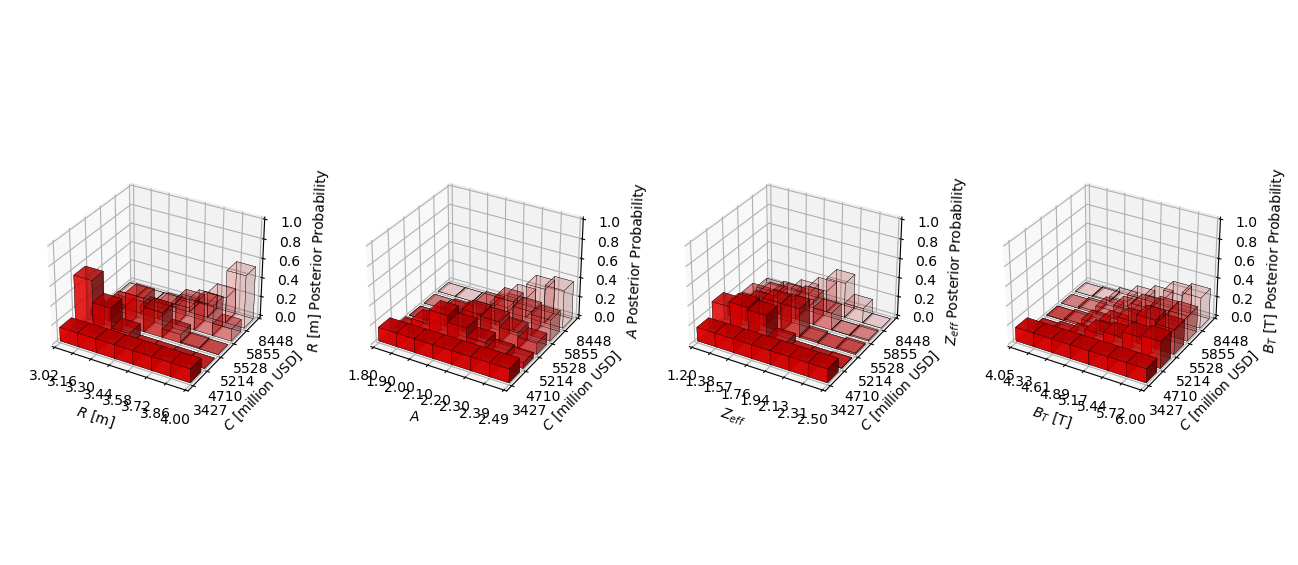
\includegraphics[width=\textwidth]{figures/TE_results/march_data/posterior_planes(RAZB)_fixed(H).png}
%     \caption{\small Posterior distributions, highlighted in red, of input parameters with changing $C$ and fixed $H$ (581--769[MWt]).}~\label{fig:posterior_planes2}
% \end{figure*}

% ~\textbf{2 outputs: $C$, $H$:} When placing evidence on $H$ ranging from 89--243 MWt and $C$ from \$3.4--4.7 billion, there were prominent updated beliefs for parameters: $R$ (3.02--3.16 m), $A$ (2.20--2.49), and $Z_{\text{eff}}$ (1.94--2.50). However, the posterior distribution of $B_{\text{T}}$ remained relatively consistent with the prior belief. 

% As $H$ increased to 243--323 MWt, $R$ exhibited greater variability (3.02--3.44m), while predictions for $A$ decreased (2.00--2.20) and $Z_{\text{eff}}$ became more pronounced (2.31--2.50). $B_{\text{T}}$ remained consistent with prior beliefs. 

% Further increasing $H$ to 323--505 MWt leads to additional shifts in the posterior distributions for input parameters. $R$ decreases and becomes more concentrated (between 3.02--3.16 m). $A$ and $Z_{\text{eff}}$ exhibit multimodal distributions, with the highest density observed at each end of the bin range and lower densities in the middle ranges [potentially indicating varying sensitivities of these parameters to changes in $H$]. Notably, $B_{\text{T}}$ alters its probable values within the range of 4.05--4.61 T, deviating from the prior distribution. 

% Beyond 505--581 MWt for $H$, the posterior distributions returned to resembling the prior distribution, indicating a limitation in establishing more probable input parameter ranges under extreme output conditions. This highlights potential challenges in accurately predicting parameter ranges under such circumstances.

% For $C$ ranging from \$4.7--5.2 billion, the highest posteriors for the given input parameters for a $H$ of 243--323 MWt were $R$: 3.44--3.86 m, $A$: 1.80--1.90, and $Z_{\text{eff}}$ 2.31--2.50. $B_{\text{T}}$ remained consistent with the prior distribution.

% As $H$ increased to 323--505 MWt, the posterior distributions for $R$, $Z_{\text{eff}}$, and $B_{\text{T}}$ shifted to lower values: 3.44--3.86 m, 1.20--1.57, 4.05--4.61 T, respectively, and for $A$, decreased to lower values between 3.44--3.86 m. 

% For $H$ of 505--581 MWt, the posterior distributions for $R$ and $Z_{\text{eff}}$ remained consistent with the prior distribution, while $A$ and $B_{\text{T}}$ exhibited multimodal distributions.

% For $H$ of 581--647 MWt, the posterior distributions for $R$ and $Z_{\text{eff}}$ remained consistent with the prior distribution, while $A$ and $B_{\text{T}}$ exhibited multimodal distributions.

To emulate a high performance reactor $E$ and $H$ were fixed to elevated values of 66--140[MWe] and 581--769[MWt], respectively. $C$ was varied in order to investigate the sensitivity input variables contingent on $C$. The analysis is split between each input parameter. Figure~\ref{fig:posterior_planes3} illustrates the posterior distributions of the input parameters with changing $C$ and fixed $E$ and $H$, where each y-axis plane represents a different $C$ value for the parameter specified on the x-axis, thus providing valuable illustrations into the sensitivity of the input parameters to changes in $C$, combined into one figure. 

\textbf{$R$} showed high sensitivity to changes in $C$. Specifically, the posterior probability density was centered between 3.02--3.30 m for $C$ of \$4.7--5.2 billion. As $C$ was increased, the probability density for $R$ shifted to increased values between 3.60--3.80m for $C$ of \$5.5--5.8 billion. When increased to the highest value of $C$, \$5.8--8.4 billion, the posterior density for $R$ lay between 3.86--4.00m. 

\text{$A$} values between 2.00--2.10 are most probable for lower $C$, \$4.7--5.2 billion. As $C$ was incrementally increased, the probability density shifted to higher values of $A$; 2.10--2.20 (for $C$ \$5.2--5.5 billion), 2.20--2.30 for $C$ of \$5.5--5.8 billion, and 2.30--2.39 for $C$ \$5.8--8.4 billion.  

\text{$Z_{\text{eff}}$} consistently showed the highest probability density between 1.20--1.76 when increasing $C$. For costs ranging \$5.8--8.4 billion, the probability density shifted increased values of $Z_{\text{eff}}$ between 1.38--1.76. This suggests that it is less sensitive to changes in $C$.

\text{$B_{\text{T}}$} remained highest within the range of 5.44--6.00 Tesla as the $C$ increased. The posterior increased in density around 5.72--6.00T with highest values of $C$. Although less pronounced than in other parameters such as $R$, this suggests that $B_{\text{T}}$ is sensitive to changes in $C$.

The posterior distributions of $R$, $A$, $Z_{\text{eff}}$, $B_{\text{T}}$ showed no sensitivity to the lowest values of $C$. This is likely due to the fact that the model is unable to predict the most probable input parameters under extreme output conditions, noting the fixed elevated values of $E$ and $H$. 

\textbf{Hybrid inference} is where evidence is placed on a combination of inputs and outputs. This is done to further understand the sensitivity of the parameters when posteriors show no sensitivity during extreme output conditions. This was done by unconstraining $C$, fixing $H$ (581--769[MWt]) and $E$ (66--140[MWe]) to emulate a high perfomance machine, and incrementally increasing $R$. The results are presented in the appendix in Figures:~\ref{fig:config(57)_outputs(3)_hybrid_2},~\ref{fig:config(57)_outputs(3)_hybrid_3},
~\ref{fig:config(57)_outputs(3)_hybrid4},~\ref{fig:config(57)_outputs(3)_hybrid5},~\ref{fig:config(57)_outputs(3)_hybrid6},~\ref{fig:config(57)_outputs(3)_hybrid7},~\ref{fig:config(57)_outputs(3)_hybrid8}.

As $R$ values were increased from between 3.02--3.16 to 3.86--4.00 the probability density of $A$ shifted from between 2.00--2.20 to increased values 2.20--2.39. For $C$ the probability density shifted, from values between \$4.7--5.2 billion, to increased values between \$5.8--8.4 billion. The probability densities for $Z_{\text{eff}}$ and $B_{\text{T}}$ remained centered around 1.57--1.94 and 5.44--6.00T, respectively, showing no shift as $R$ was increased. 

% ~\textbf{4 outputs}: Here, the aim was to emulate the highest performing reactor system possible, with the addition of a fourth output, $Q_{\text{eng}}$. This meant fixing $E$, $H$ and $Q_{\text{eng}}$ to elevated values of 66--140[MWe] and 581--769[MWt], and 1.40--1.90 respectively, and varying $C$ in order to investigate the sensitivity input varibles contingent on $C$. 

% For $C$ values ranging between \$5.5--5.8 billion, the posterior distributions of $R$ were highest between 3.72--4.00 m (showing a prominent peak betwen 3.86--4.00 m), $A$ between 2.20--2.49, $Z_{\text{eff}}$ between 1.76--1.94, and $B_{\text{T}}$ between 5.17--6.00T. When reducing $C$, the posterior distributions of $R$, $A$, $Z_{\text{eff}}$ and $B_{\text{T}}$ showed no sensitivity with the specified fixed ranges other outputs. This occured for any ranges of $C$ below \$5.5--5.8 billion. As with the 3-output model, this is likely due to the fact that the model is unable to predict the most probable input parameters under extreme output conditions, noting the fixed elevated values of $E$, $H$, and $Q_{\text{eng}}$.

% In order to further understand the sensitivity of the input parameters, the extreme conditions of the outputs were lessened by reducing the value for $Q_{\text{eng}}$ to 1.10--1.40. $C$ was further reduced to \$5.2--5.5 billion, while $H$ and $E$ remained fixed. The posterior distributions of $R$ showed similar results to above, and were highest between 3.44--3.72 m (with less of a promient peak in the 3.86--4.00 range). For $A$ and $Z_{\text{eff}}$ the postreriors shifted to higher values between 2.30--2.49 and 1.94--2.13, respectively. For $B_{\text{T}}$ posteriors shifted to lower values between 4.89--5.72T.

% Further reductions in $C$ resulted in the posterior distributions of $R$, $A$, $Z_{\text{eff}}$ and $B_{\text{T}}$ showing no sensitivity with the outputs under extreme conditions, noting the fixed elevated values of $E$, $H$, and $Q_{\text{eng}}$.

\section{Discussion}\label{sec:Discussion}

%%\subsection{Forward Inference}\label{sec:disc_forward}

\subsection{Reverse Inference}\label{sec:disc_reverse}

The outcomes of the reverse inference analysis provide fusion developers with valuable insights into optimising the design parameters of fusion reactors and their components. The ability to identify the most probable input parameters for a given set of output parameters, can significantly inform the design process. By examining the posterior distributions of fusion input parameters in relation to specified output parameters, such as elevated values of energy output ($E$), fusion power ($H$), and $Q_{\text{eng}}$, developers can identify the most probable input parameter ranges that lead to high-performance reactor systems. The results highlight the ability to use the model across different stages of the design process, and it is expected to provide valuable insights for the development of future fusion power plants. In addition, the ambiguity of the model and its ability to handle data from any input-output model highlight the flexibility and adaptability of the BN, making it a valuable tool for fusion developers.

The observed sensitivity of key input parameters, namely $R$, $A$, $Z_{\text{eff}}$, and $B_{\text{T}}$, to changes in $C$ provide crucial depth in analysis for the developer. The variations in the probability density distributions suggest nuanced considerations in reactor design optimisation, particularly concerning cost-performance trade-offs. 

\begin{figure*}[t]
    \centering
    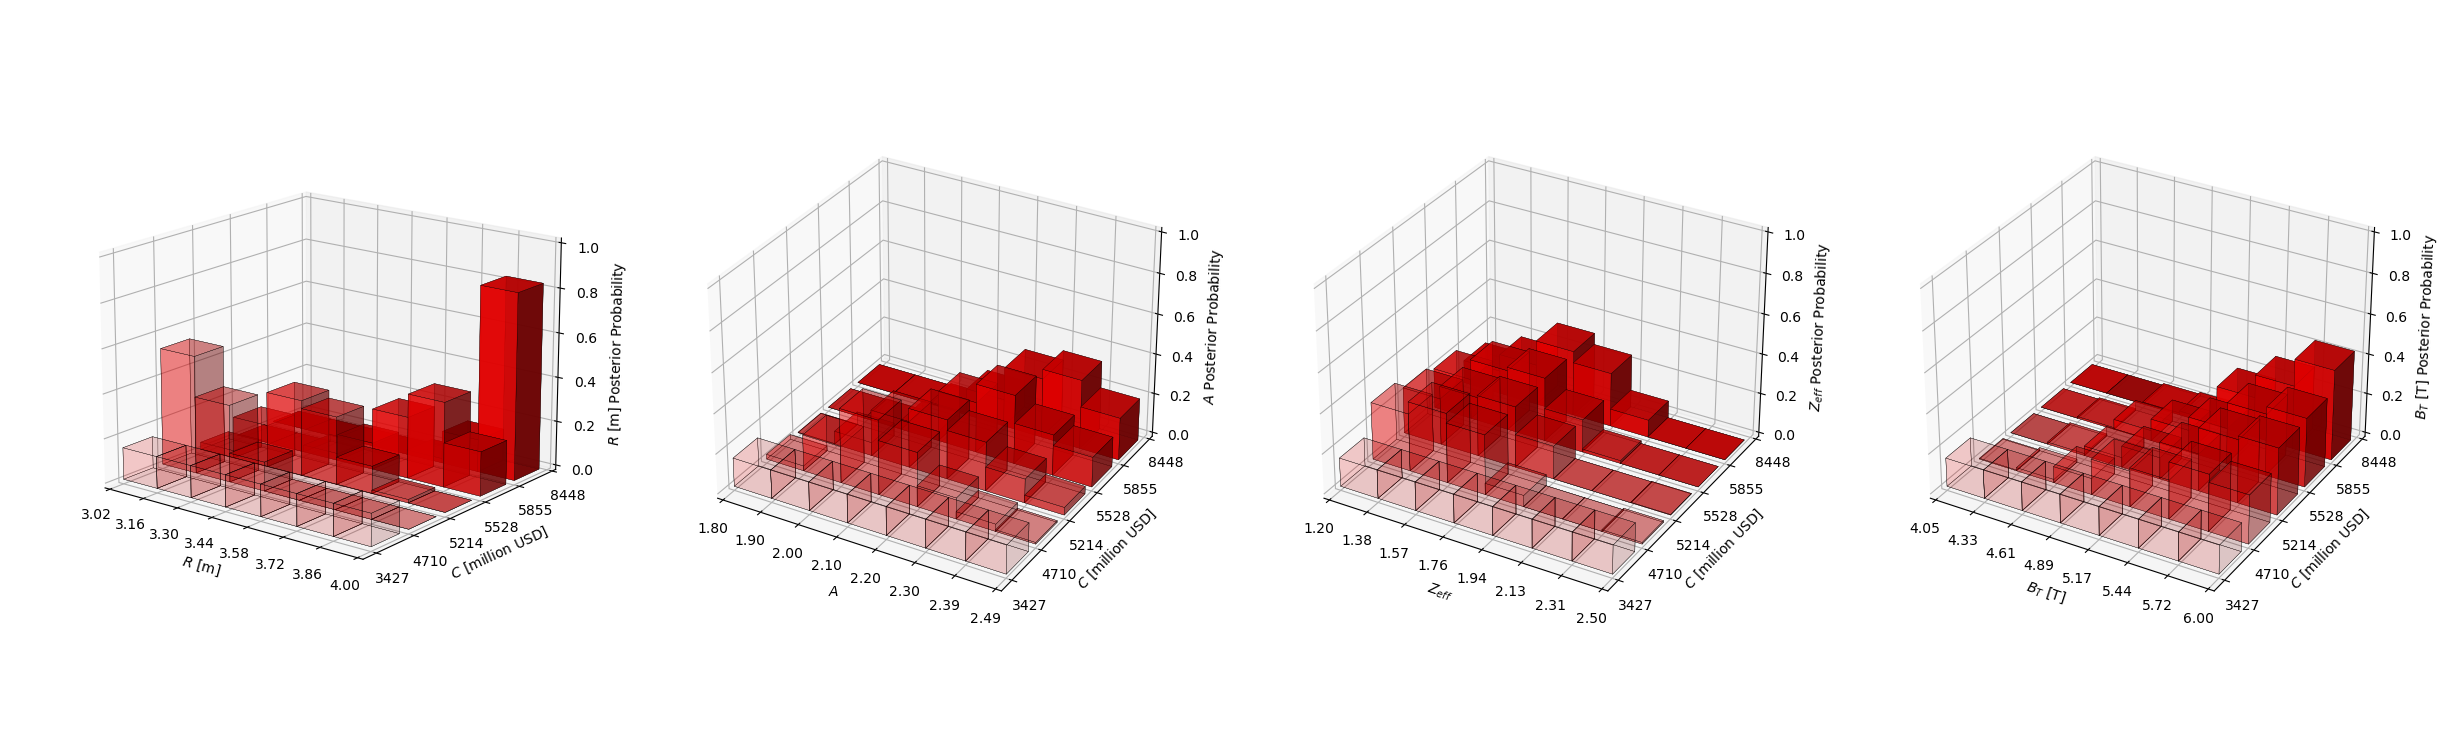
\includegraphics[width=\textwidth]{figures/TE_results/march_data/3D_posteriors.png}
    \caption{\small Posterior distributions, highlighted in red, of input parameters with changing $C$ and fixed $H$ (581--769[MWt] and $E$ (66--140[MWe])).}~\label{fig:posterior_planes3}
\end{figure*}

\textbf{$R$}: The observed sensitivity of the $R$ to changes in $C$, in both reverse and hybrid inference analysis, as indicated by shifts in posterior probability density distributions, underscores the intricate relationship between fusion reactor design parameters and construction expenses. While it may seem intuitive that larger machines with greater major radii would inherently entail higher construction costs, the significance lies in the ability of the probabilistic model to capture and quantitatively represent this relationship. It affirms that the probabilistic framework effectively captures the underlying dynamics and dependencies within the fusion system. 

Insights derived from the probabilistic analysis can inform optimisation strategies aimed at balancing performance objectives with cost considerations. By identifying the trade-offs between major radius, construction cost, and other design parameters, engineers can explore design alternatives that optimise both technical performance and economic feasibility.

\textbf{$A$}: Similarly, the variation in the most probable $A$ values in response to changes in $C$ reflects the intricate balance between geometry and economic feasibility. Lower-cost machines favour lower $A$, indicating potential design adjustments to optimise cost-effectiveness with no compromise in performance. Increasing the $R$ of an ST typically requires an increase in the $A$ to maintain stability and confinement efficiency in the plasma~\cite{Costley2021}. However, it's essential to note that the relationship between $R$ and $A$ depends on various factors, including the specific design objectives, engineering constraints, and plasma physics considerations. Engineering constraints, such as the available space, manufacturing capabilities, and material requirements, play a significant role in determining the relationship between $R$ and $A$~\cite{Costley2021}. Manufacture of an ST with a larger $R$ may necessitate adjustments in the $A$ to ensure compatibility with existing infrastructure and manufacturing processes. 

$A$ also influences the plasma physics in ST designs. For example, STs typically have less space in the central solenoid, limiting the ability for self start up, therefore requiring additional heating methods. For example, neutral beam injection (NBI) -one method of additional heating- means that the aspect ratio has to be [higher/lower?], whereas electron cyclotron resonance heating (ECHR) means that $A$ has to be [higher/lower?] [THESE QUESTIONS TO BE ANSWRED BY TE AS THEY ARE LOOKING TO USE ECRH]. It should be noted that increasing the major radius while maintaining a specific aspect ratio may involve trade-offs in reactor performance, cost, and complexity. Balancing these factors to optimize reactor performance will be key to meeting project requirements and budget constraints. Therefore, while higher $A$ might indeed be necessary for larger STs, this relationship is not absolute and may vary depending on the specific design requirements and trade-offs.

\text{$Z_{\text{eff}}$}: Contrastingly, the consistent probability density distribution of $Z_{\text{eff}}$ across different $C$ ranges suggests a relative insensitivity of this parameter to economic considerations. This could be due to several reasons. The behaviour of $Z_{\text{eff}}$ is governed by intrinsic plasma characteristics and operating conditions, which remain relatively constant across different $C$ scenarios. As a result, variations in $C$ do not significantly influence $Z_{\text{eff}}$. The design and optimisation process may prioritise achieving target values or ranges for $Z_{\text{eff}}$ to ensure optimal plasma performance. Consequently, adjustments in $C$ to meet economic constraints may not directly impact the underlying plasma properties represented by $Z_{\text{eff}}$. The observed insensitivity of $Z_{\text{eff}}$ to changes in $C$ could reflect the robustness of the fusion system design in maintaining desired plasma characteristics under vAarying economic conditions. This suggests that the relationship between $Z_{\text{eff}}$ and $C$ may be influenced by factors beyond direct economic considerations. The complex interplay of various factors within the fusion system, including plasma physics, engineering constraints, and operational requirements, may lead to emergent behaviours where changes in $Z_{\text{eff}}$ have limited direct impact on $C$, or vice versa.

\text{$B_{\text{T}}$}: The increasing probability density of $B_{\text{T}}$ with higher $C$s underscores the significance of toroidal field strength in larger STs. This observation emphasizes the pivotal role of magnetic confinement in accommodating larger plasma volumes and achieving sustained fusion reactions at scale. 

In STs, the requirement for higher magnetic field strengths necessitate the use of high-temperature superconducting (HTS) magnets. HTS magnets offer significant advantages in terms of efficiency and strength but are also more complex and expensive to manufacture. The production and installation of these advanced magnet systems can substantially contribute to the overall capital cost of the fusion reactor. Additionally, the development and deployment of HTS technologies require substantial research and development investments, specifically where performance under high neutron fluxes are concerned. 

Increasing $B_{\text{T}}$ may require optimisation of components to accommodate the higher magnetic field. For instance, the vacuum vessel, plasma-facing components, and diagnostic systems may require reinforcement to withstand the increased magnetic forces associated with higher $B_{\text{T}}$. 

In addition, variations in $B_{\text{T}}$ directly impact plasma confinement and stability. Achieving and maintaining higher $B_{\text{T}}$ levels will need to address challenges such as plasma disruptions, instabilities, and heat loads on plasma-facing components. In addition, the optimisation of magnet configurations will need to be addressed. This will involve designing efficient cooling systems for superconducting magnets, and ensuring compatibility with other reactor components. 

The lack of sensitivity of the posterior distributions of $R$, $A$, $Z_{\text{eff}}$, and $B_{\text{T}}$ to the lowest values of $C$ suggests that the model may face limitations in predicting the most probable input parameters under extreme output conditions. This phenomenon could be attributed to several factors. Firstly, the fixed elevated values of $E$ and $H$ may constrain the range of feasible solutions, thereby limiting the variability in the input parameters. In other words, when the desired output parameters are set at relatively high levels, the model may prioritize fulfilling these requirements, potentially constraining the flexibility in selecting input parameters such as $R$, $A$, $Z_{\text{eff}}$, and $B_{\text{T}}$. 

Consequently, the posterior distributions of these input parameters may exhibit reduced sensitivity to variations in the lowest values of $C$. Furthermore, it's possible that the model's training data or assumptions may not adequately capture the complex interdependencies and trade-offs between input and output variables under extreme conditions. As a result, the model may struggle to accurately predict the most probable input parameters when the output conditions are set at extreme levels. Overall, the observed lack of sensitivity underscores the importance of carefully validating and calibrating the model, as well as considering the range of output conditions when interpreting the results of the techno-economic analysis. Further refinement of the model, possibly through incorporating additional data or refining the model's algorithms, may help improve its predictive capabilities under extreme output conditions.

% 4 outputs: 

% The analysis reveals a significant shift in the most probable input parameters for fusion reactor design, contingent upon the reactor's $C$. For reactors with a lower $C$ (\$3.2--3.8 billion), optimal parameters tend towards a smaller $R$, higher $Z_{\text{eff}}$, and lower $B_{\text{T}}$, aligning with specified output parameter ranges. The posteriors of $A$ illustrates a broader distribution compared to other input parameters. This suggests that for lower $C$ machines, there is increased flexibility in selecting the desired value for $A$. However, as $C$ is increased (\$4.4--6.5 billion), the most probable parameters shift, indicating a need for a larger $R$, reduced $A$, reduced $s_{\text{eff}}$, and increased $B_{\text{T}}$ to meet the specified output parameters.

% The observed decrease in $A$ with increased $C$ can be interpreted through the lens of engineering trade-offs. As $C$ rises, design considerations may prioritise aspects like scalability and efficiency over compactness. A larger $R$ accommodates more plasma volume, potentially enhancing overall reactor performance and output, albeit at the expense of increased material and construction costs. Moreover, a lower $A$ may be favored in larger-scale reactors to optimise plasma stability and confinement, aligning with the operational demands of a higher-budget project. 

% This model-based insight underscores the intricate interplay between reactor design parameters and capital investment. The shift in optimal parameters with varying $C$s highlights the nuanced considerations that developers must navigate to achieve cost-effective and high-performance fusion reactor designs. By interpreting these results, developers can strategically tailor design choices for reactor components, such as toroidal magnets and vacuum vessels, to optimise performance within budgetary constraints, fostering advancements in fusion energy technology.

\section{Conclusion and Further Work}\label{sec:conc}

These insights enable developers to make informed decisions during the design optimisation process, especially for reactor size and geometry. By focusing on the input parameter ranges associated with high $E$ and $H$ minimal $C$ it is possible to enhance performance while considering cost constraints. This probabilistic framework can guide the selection of input parameters to achieve specific performance targets within budgetary limitations. It is important to note that these results are based on the current state of knowledge and technology. As such, it would be beneficial to continually update the BN as new data becomes available. This could include results from experiments, advancements in plasma physics, or changes in manufacturing costs.

Probabilistic Bayesian inference serves as a powerful tool for enhancing fusion research by providing a comprehensive framework for integrating data, quantifying uncertainties, optimising experimental design, supporting decision-making, and managing risks. By leveraging Bayesian methods in conjunction with existing approaches, fusion researchers can gain deeper insights into reactor behaviour, accelerate the pace of innovation, and advance the development of practical fusion energy solutions.

\section{Acknowledgments}
This research was supported by the EPSRC (Engineering and Physical Sciences Research Council, UK) Nuclear Energy Futures Centre for Doctoral. Training in Nuclear Energy (NEF CDT). Other research studies under the NEF CDT involving Thomas Griffiths are supported in part by Tokamak Energy Ltd, UK.\ Views and opinions expressed are however those of the author(s) only and do not necessarily reflect those of Tokamak Energy Ltd.


\bibliographystyle{IEEEtranN}
\bibliography{library}

\begin{appendices}
    \section{Appendix: Prediction Accuracy}\label{appendix:prediction_accuracy}

\begin{table}[h]
    \centering
    \resizebox{\columnwidth}{!}                         \\ \cline{3-8} 
    \multicolumn{2}{|l}{}                                                           & \multicolumn{3}{c|}{$d_{1}$} & \multicolumn{3}{c|}{$d_{2}$}                   \\ \hline
    \multicolumn{2}{|c|}{Dataset size} &
        \multicolumn{1}{l|}{1400} &
        \multicolumn{1}{l|}{5120} &
        \multicolumn{1}{l|}{10240} &
        \multicolumn{1}{l|}{1400} &
        \multicolumn{1}{l|}{5120} &
        10240 \\ \hline
    \multicolumn{1}{|c|}{\multirow{3}{*}{Bin resolution}} & \multicolumn{1}{l|}{5}  & 92.73  & 92.84  & 93.13 & 96.36 & 96.76                     & 96.73 \\ \cline{2-2}
    \multicolumn{1}{|c|}{}                                & \multicolumn{1}{l|}{7}  & 93.74  & 94.08  & 94.79 & 96.98 & 96.79                     & 97.00 \\ \cline{2-2}
    \multicolumn{1}{|c|}{}                                & \multicolumn{1}{l|}{10} & 89.37  & 91.20  & 90.86 & 88.25 & \multicolumn{1}{r}{89.75} & 89.40 \\ \hline
    \end{tabular}%
    }
    \caption{\small A table displaying the average accuracy of predictions for $d_{1}$ and $d_{2}$ errors while investigating variations in both (i) the size of the dataset and (ii) the resolution of bins.}
    \label{tab:prediction_accuracy}
\end{table}

\begin{figure*}[h]
    \centering
    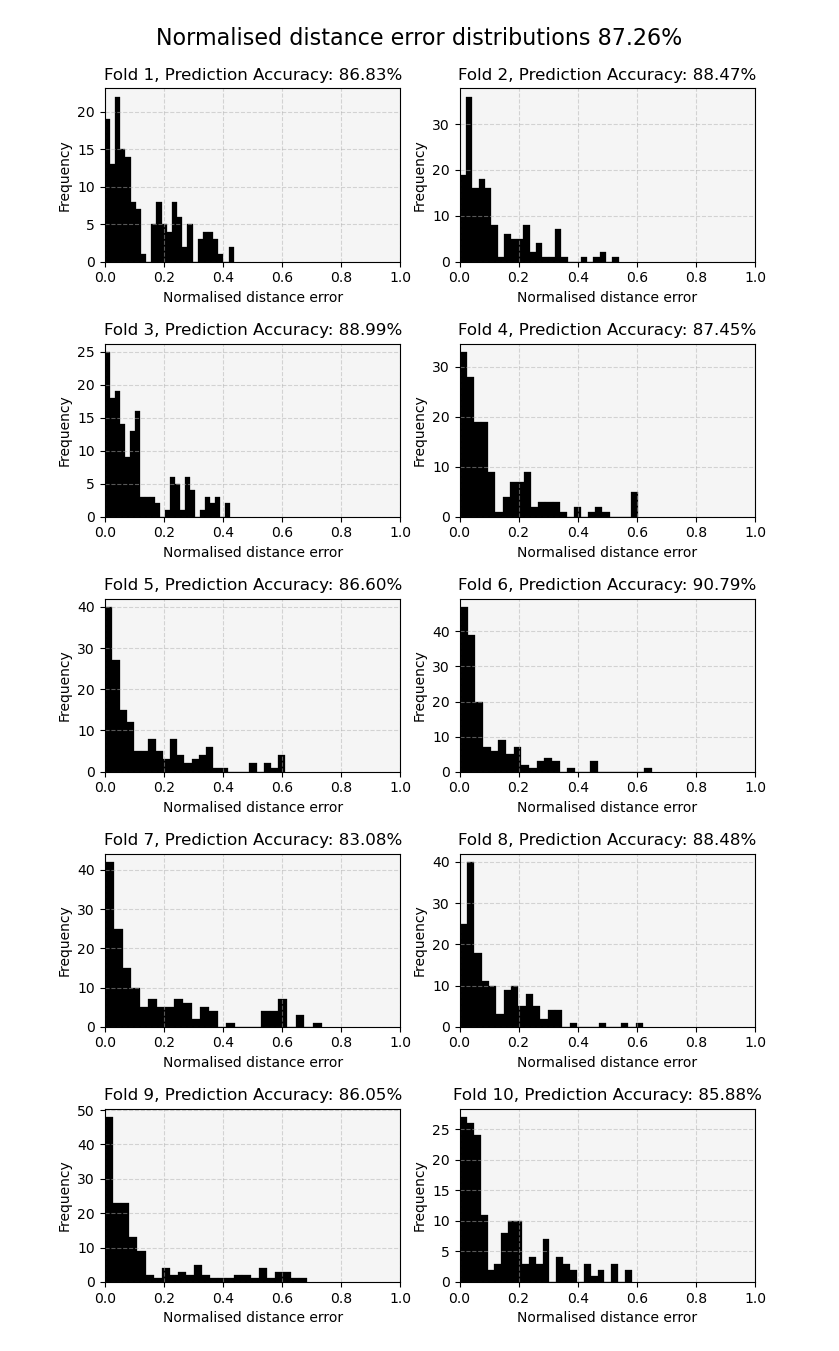
\includegraphics[width=0.65\textwidth]{figures/validation_plots/TE/k-fold_two_outputs.png}
    \caption{\small Normalised probability histograms with prediction accuracy values for each fold is shown for $d_{1}$ bin configuration: inputs (7) outputs (5), dataset size = 10240.}~\label{fig:k-foldhistogramsTE}
\end{figure*}
 \end{appendices}

\end{document}